% ----------------------------------------------------------------------^
% Copyright (C) 2004, 2005, 2006, 2007, 2008, 2009 
% Giorgio Calderone <gcalderone@ifc.inaf.it>
% 
% This file is part of DIF.
% 
% DIF is free software; you can redistribute it and/or modify
% it under the terms of the GNU General Public License as published by
% the Free Software Foundation; either version 2 of the License, or
% (at your option) any later version.
% 
% DIF is distributed in the hope that it will be useful,
% but WITHOUT ANY WARRANTY; without even the implied warranty of
% MERCHANTABILITY or FITNESS FOR A PARTICULAR PURPOSE.  See the
% GNU General Public License for more details.
% 
% You should have received a copy of the GNU General Public License
% along with DIF; if not, write to the Free Software
% Foundation, Inc., 51 Franklin St, Fifth Floor, Boston, MA  02110-1301  USA
% 
% ----------------------------------------------------------------------$


\documentclass[10pt,titlepage]{article}

\usepackage[english]{babel}
\usepackage{graphicx}
\usepackage{framed}
\usepackage{listings}
\usepackage{url}
\usepackage{a4wide}
\usepackage{fancyhdr}
\pagestyle{fancy}
\renewcommand{\footrulewidth}{0.4pt}

%LN
%\renewcommand{\sectionmark}[1]{\markright{\thesection.\ #1}}
%\renewcommand{\sectionmark}[1]{\markright{#1}}
%\renewcommand{\subsectionmark}[1]{\markright{#1}}
%\parindent 0pt


%\textheight 22cm
%\textwidth 16.5cm
%\topmargin 0cm
%\oddsidemargin -0.5cm
%\evensidemargin -0.5cm
%\sloppy
 
\def\deg{^\circ}
\def\fdeg{\hbox{$\,.\!\!^{\circ}$}}
\newcommand{\dif}{\textbf{\small DIF}}

\def\ver{Ver. \input{../version}}
%\def\url{http://ross.iasfbo.inaf.it/MCS/}

\newcommand{\syntax}[1]
{
  \bigskip
  \noindent
  \textbf{Syntax:} \\ 
  \indent \texttt{#1}
}

\newenvironment{parameters}
{
  \medskip
  \noindent
  \textbf{Parameters:}
  \begin{enumerate}
}
{
  \end{enumerate}
}

\newcommand{\param}[2]
{
  \item \textit{#1} \texttt{#2} 
}

\newcommand{\return}[1]
{
  \medskip
  \noindent
  \textbf{Return value} (\texttt{#1}): \\
  \indent
}

\newcommand{\example}
{
\medskip
\noindent{\textbf{Example:}}
}

\lstloadlanguages{SQL}
\lstset{
  basicstyle=\scriptsize\ttfamily
  ,captionpos=b
  ,float=hbt
  ,frame=trBL
  ,language=SQL
  ,keywordstyle=\bfseries, stringstyle=\ttfamily, commentstyle=\textit,
  emph={
    TINY,SMALL,MEDIUM,INT,BIGINT,FLOAT,DOUBLE,STRING,TIME,TINY_BLOB,BLOB
    ,AccumBuffer}
}
%
%

\begin{document}
\title{
%
\textbf{DIF \\ Dynamic Index Facility}
%
%\thanks{\url}
%
%\begin{center}
%\vspace{0.8cm}
%\includegraphics[width=5cm,keepaspectratio]{mcslogo} \\
%\vspace{0.8cm}
%\end{center}
%
\centerline{\rule{\textwidth}{0.4pt}}
%
}
\bigskip
\author{
  \sc{Giorgio Calderone} \\
  %\footnote{Giorgio Calderone $<$gcalderone@ifc.inaf.it$>$}  \\
  \sc{INAF - Trieste Observatory, Italy} \\ \\
  \sc{Luciano Nicastro} \\
  %\footnote{Luciano Nicastro $<$nicastro@iasfbo.inaf.it$>$} \\
  \sc{INAF - IASF Bologna, Italy} \\
 }
%\date{\today \\
\date{August 5, 2016 \\
      \ver \\
      \url{http://ross.iasfbo.inaf.it/MCS/} \\
      \centerline{\rule{\textwidth}{0.4pt}}
     }
\maketitle

\thispagestyle{empty}
~

\vfill
{\it\small This page intentionally left blank.}

\newpage
\pagenumbering{roman}

\tableofcontents

\newpage
\pagenumbering{arabic}
%\mainmatter

%
%
%---------------------------------------------------------------------
\newpage

\section{Introduction}
Typically DB server offer efficient indexing of one or more 1--d data
using the so called B--tree structure. Data produced by an
astronomical experiment however are typically related to sky
coordinates which span a 2--d space. Although it is possible to index
such data using one or two simultaneous 1--d indexes like RA and Dec,
the queries performance will be very poor since the search criteria on
a 2--d space can be much more complex than on an union of two
independent 1--d spaces. Indeed the only possible queries that take
advantages of such indexes will involve range checking along the two
coordinates: $\alpha_1 \le \alpha \le \alpha_2$ and $\delta_1 \le
\delta \le \delta_2$. In some cases, the DB server provides built-in
capabilities to manage 2--d coordinates into indexes using the R--tree
structure. This would allow search criteria like ``Find all objects
within 2 arcsec of a given location''. However these functionalities
are far from being a standardized feature of DB servers; furthermore,
there is room for optimization and specialization for astronomical
usage.

\bigskip

\dif\ is a set of tools aimed at implementing a powerful indexing
system for astronomical catalogues, or any other table containing spherical
coordinates, stored into MySQL databases. It
uses a sphere pixelization scheme to convert a latitude/longitude coordinate
system into a single pixel ID, and creates a B--tree (1--d) index on
it. Furthermore it provides a number of functions to generate the
pixel IDs given a search criteria such as ``Find all the objects within
a given cone''. This way it allows very fast queries
execution even on billion-rows tables, using the MySQL built-in
indexing system. \dif\ provides two pixelization schemas:
HTM\footnote{\url{http://www.sdss.jhu.edu/htm/}} and
HEALPix\footnote{\url{http://healpix.jpl.nasa.gov/}} (with either RING
or NESTED map ordering). \dif\ software and documentation is distributed
as an open source package under the GPL license at the site
\url{http://ross.iasfbo.inaf.it/MCS/}. Please note that though tested
and operational, this package is continuosly updated and relevant
changes could affect new versions. Please keep checking the web
site. Should you find any bug or inconsistency, or if you wish to
suggest new features and/or contribute to the development, please
write us at:

\begin{itemize}
\item Giorgio Calderone $<$calderone@oats.inaf.it$>$
\item Luciano Nicastro $<$nicastro@iasfbo.inaf.it$>$
\end{itemize}
%

\bigskip
This document is organized as follows: \S\ \ref{sec:pixschema}
provides an overview of the HTM and HEALPix pixelization schemas.
\S\ \ref{sec:install} shows how to install \dif, whereas
\S\ \ref{sec:usage} shows how to use it. \S\ \ref{sec:howitworks}
describes \dif\ internals and \S\ \ref{sec:bench} provides some guideline
on how to reach good performance in queries excecution. Finally
\S\ \ref{sec:DIF_function_reference} provides the reference to all the
\dif\ related functions.


%The main software
%components of \dif\ are:
%%
%\begin{enumerate}
%\item a Perl script used to perform administrative tasks;
%\item a C++ library which implemets the \dif\ DB engine;
%\item a set of SQL and SQL callable C++ functions;
%\end{enumerate}
%Once \dif\ has been installed its use is completely trasparent to the
%MySQL users.
%
%\smallskip
%
%
%

\subsection{What's new in version 0.5.4}
\begin{itemize}
\item Replaced HEALPix C++ library with version 3.30.
\item Added rectangular region selections for HEALPix indexed tables.
\item Added \texttt{HEALPBound} and \texttt{HEALPBoundC} UDFs.
\item Added \texttt{difview\_htmClean}, \texttt{difview\_healpClean},
 \texttt{difview\_Check} and \texttt{difInfo} SQL procedures.
\item Added \texttt{DIF.func} table.
\item The \texttt{dif} script uses new default settings and has more options
 and commands. In particular, as root, it is possible to grant minimal
 privileges to users in order to be able to manage specific DBs.
 See \texttt{dif -h}.
\item Code cleaning.
\item Documentation updated.
\end{itemize}


\subsection{What's new in version 0.5.3}
\begin{itemize}
\item  Works also for MySQL 5.6 and 5.7 (and MySQL Cluster 7.2 and MariaDB 10.0, 10.1).
\item  Use memset instead of bzero.
\item  Added UDF \texttt{HTMsNeighb} and DIF function \texttt{DIF\_sNeighb}
  to get higher depth trixels around a given trixel.
\item  \texttt{dif} script update with additional options (see \texttt{dif -h}).
\item  Documentation updated.
\end{itemize}


\subsection{A simple example}
Once \dif\ is installed (\S\ \ref{sec:install}) a database named
{\tt DIF} will be created, with a test table named {\tt Messier}
in it. This
table simply contains the Messier catalogue of astronomical objects. Its purpose
is to test \dif\ functionalities before using it to real data tables. The
equatorial coordinates in degrees of each object are stored in the
{\tt Ra} and {\tt Decl} fields (note that MySQL does not allow to have an
``unquoted'' field named {\tt Dec} because it is a reserved word -- it is a synonym for
{\tt DECIMAL}). To create a HTM index with depth 6
(see \S\ \ref{sec:pixschema}) simply issue the command:
\begin{verbatim}
  dif --index-htm DIF Messier 6 Ra Decl
\end{verbatim}
Now you can query the DB server requesting, for example, all the objects in
the catalogue within 100 arcmin from the point with Ra = $82\deg$,
Dec = $22\deg$:
\begin{lstlisting}[
    caption={Check \dif\ functionality on Messier table.},
    label={lst_check}]
mysql> SELECT * FROM Messier_htm_6 WHERE DIF_Circle(82, 22, 100);
+---+------+-------+------+--------+---------+---------+---------+-----------+--------+
| M | Type | Const | Mag  | Ra     | Decl    | Dist    | htmID_6 | HTM_Depth |HTM_Full|
+---+------+-------+------+--------+---------+---------+---------+-----------+--------+
| 1 | BN   | Tau   |  8.2 | 83.625 | 22.0167 | 6.3 kly |   62340 |         6 |       0|
+---+------+-------+------+--------+---------+---------+---------+-----------+--------+
1 row in set (0.00 sec)
\end{lstlisting}
%

%\newpage
\section{The HEALPix and HTM pixelization schemas}
\label{sec:pixschema}
The HEALPix pixelization scheme (G\'orski et al., ApJ 662, 759, 2005)
uses equal-area pseudo-square pixels,
particularly suitable for spatial analysis.
The base pixels are 12 with two different shapes (Fig. \ref{fig:sphPix}).
The region in the range $-2/3< z < 2/3$ is referred as
the equatorial zone, the two remaining regions being the polar caps.
Recursive subdivision of these pixels is performed keeping their centers
equally distributed along rings of constant colatitude. Rings located in the
equatorial zone are divided into the same number of pixels; the remaining
rings contain a varying number of pixels.  The two rings closest to the poles
always have 4 pixels and going toward the equator the number of pixels
increases by 4 at each step. The resolution of the HEALPix grid is
parameterized by $N_{\rm side} = 2^k$, where $k$ assumes integer values being
0 for the base pixelization. It is called the ``resolution parameter'' or
\emph{order}. It is then $N_{\rm pix} = 12\times N_{\rm side}^2$.
The HEALPix library implements a recursive
quad-tree pixel subdivision which is naturally nested.  The resulting pixel
numbering scheme is then referred as the \emph{nested} scheme. Alternatively
the \emph{ring} scheme simply counts the pixels moving down from the north to
the south pole along each isolatitude ring (see Fig. \ref{fig:sphPix}).
The usage of the ring scheme is not recommended to index tables like object
catalogues which are typically queried on small sky regions. In fact in this
case a pixel ID-bind data sorting will not result into an efficient
``grouping'' like that obtainable for the nested scheme where to
``close-on-sky'' pixels correspond ``close-on-disk'' data.
This is an important issue because data seek time is the main issue to face
when dealing with very large tables.

The HTM sphere pixelization scheme (Kunszt et al., 2001)
uses triangular pixels which can
recursively be subdivided into four pixels. The base pixels are 8.
They are obtained by the intersection on the sphere of 3 major big
circles. On the Earth they can be represented by the equator and two meridians
passing at longitude $0\deg$ and $90\deg$ (see Fig. \ref{fig:sphPix}).
These
base spherical triangles all have the same area.  Each of them can then be
further divided into four spherical triangles, or \emph{trixels}, by
connecting the three sides middle points using great circle segments. As can
be seen from Fig. \ref{fig:sphPix}, from the first subdivision onward the
resulting trixels
are no longer equal-area. The scatter of the trixels area remains within the
$\pm70\%$ of the mean area, which is $2\pi/4^{d+1}$, being $d$ the
\emph{depth} or level (step of recursive subdivision) of the trixel.  For a
given depth the number of trixels is $N_{\rm pix} = 8\times 4^d$.  The minimal
side length is $\pi/2^{d+1}$ and the maximal is $\simeq \pi/2$ times the
minimal length.

The relevant parameters for the two pixelizations are reported in Table
\ref{tab:1}.
%
%--
\begin{table}[tbp]
\centering
\caption{Relevant parameters for the HTM and HEALPix sphere pixelization}
\label{tab:1}
%\begin{center}
\begin{tabbing}
%
Max res.$^*$ ($^{\prime\prime}$): \= $[N_{\rm pix} , 2\times N_{\rm pix}-1]$ \=
~~ \= $12 \times N_{\rm side}^2$ (where $N_{\rm side} = 2^k$) \kill

 \> \textbf{HTM}  \> \> \textbf{HEALPix}  \\
$N_{\rm pix}^\dagger$: \> $8\times 4^d$ \> \>
   $12 \times N_{\rm side}^2$ (where $N_{\rm side} = 2^k$)\\
ID range: \> $[N_{\rm pix}\;, 2\times N_{\rm pix}-1]$ \> \>
     $[0\;, N_{\rm pix}-1]$ \\
Max $N_{\rm pix}$: \> $\simeq 9.0\times 10^{15}$ \> \> $\simeq 3.5\times
10^{18}$ \\
Max res.$^*$ ($^{\prime\prime}$): \> $\simeq 1\times 10^{-2}$ \> \> $\simeq 4\times
10^{-4}$
 ($\Omega_{\rm pix} = \pi/(3\times N_{\rm side}^2)$) \\
%
%\hbox{\rule{\textwidth}{0.4pt}}
\rule{100pt}{0.4pt}
\\
$^\dagger d$ (depth): $[0\;, 25]$; ~
 $k$ (order $\Leftrightarrow$ resolution parameter): $[0\;, 29]$ \\
$^*$ For HTM the maximum resolution is derived from the trixel minimum side, \\
~ for HEALPix assuming a square-pixel equivalent area.
\end{tabbing}
%\end{center}
\end{table}
%
We, in general, suggest to
prefer the HTM pixelization because it offers a larger set of functions with
respect to HEALPix. We'll see below that the HEALPix IDs of any set of
selected rows can still be computed using the DIF functions at query execution
time.

\begin{figure}[btp]
\centering
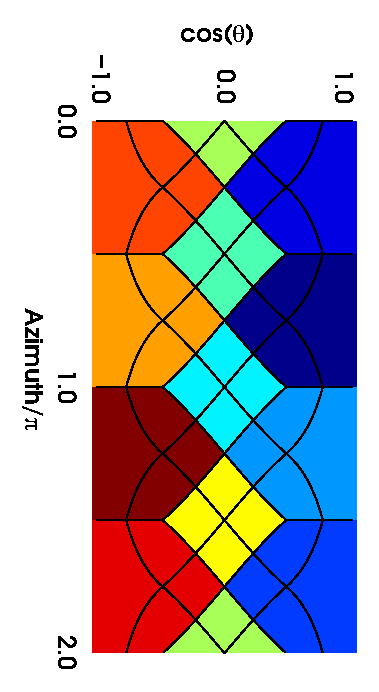
\includegraphics[height=5cm,angle=90,clip=]{includes/hpx_cart}
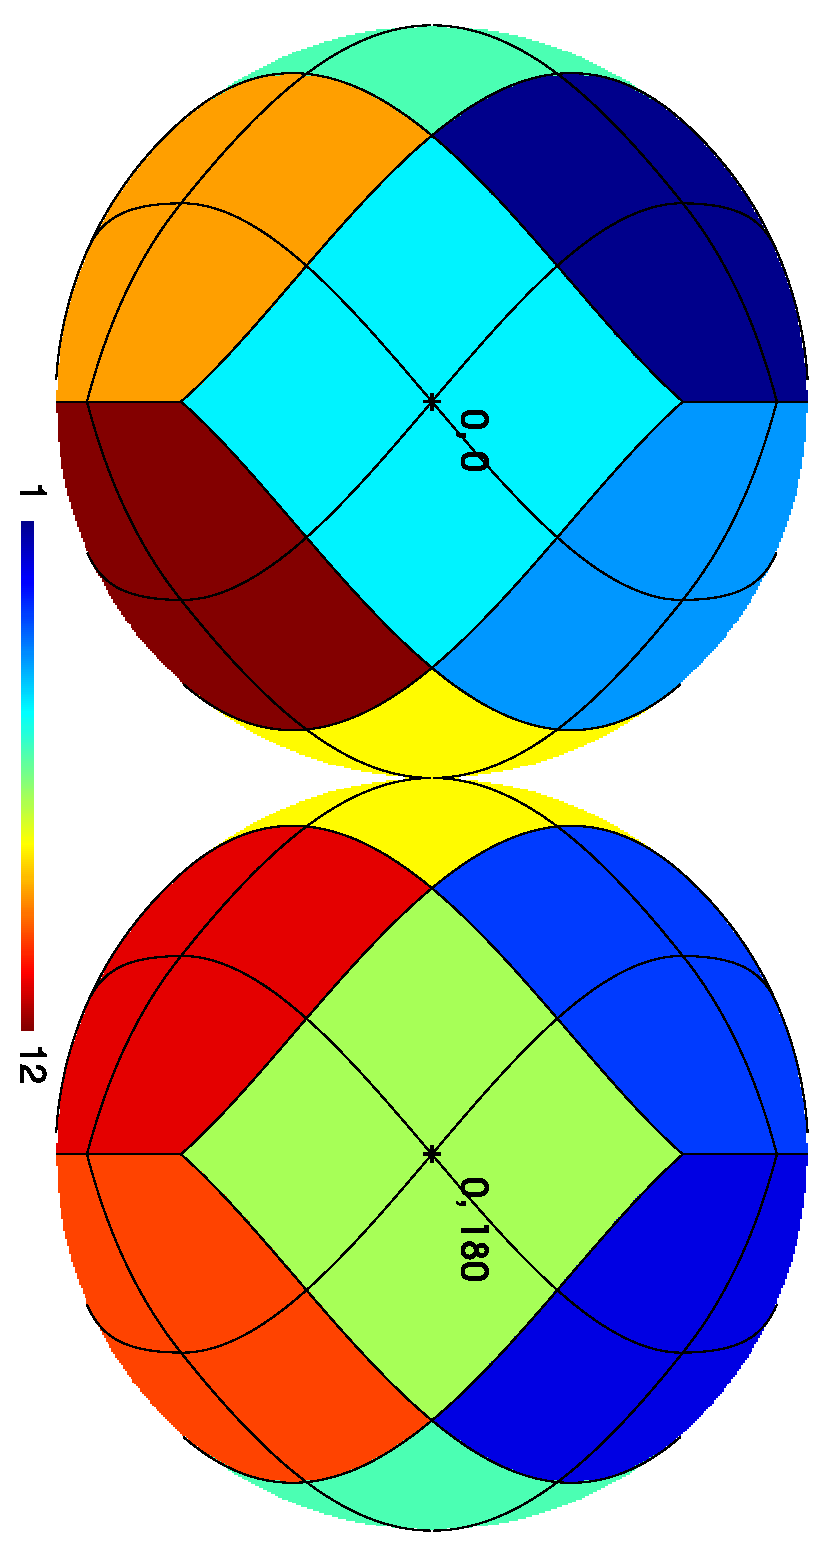
\includegraphics[height=5.5cm,angle=90,clip=]{includes/hpx_draw_k0}
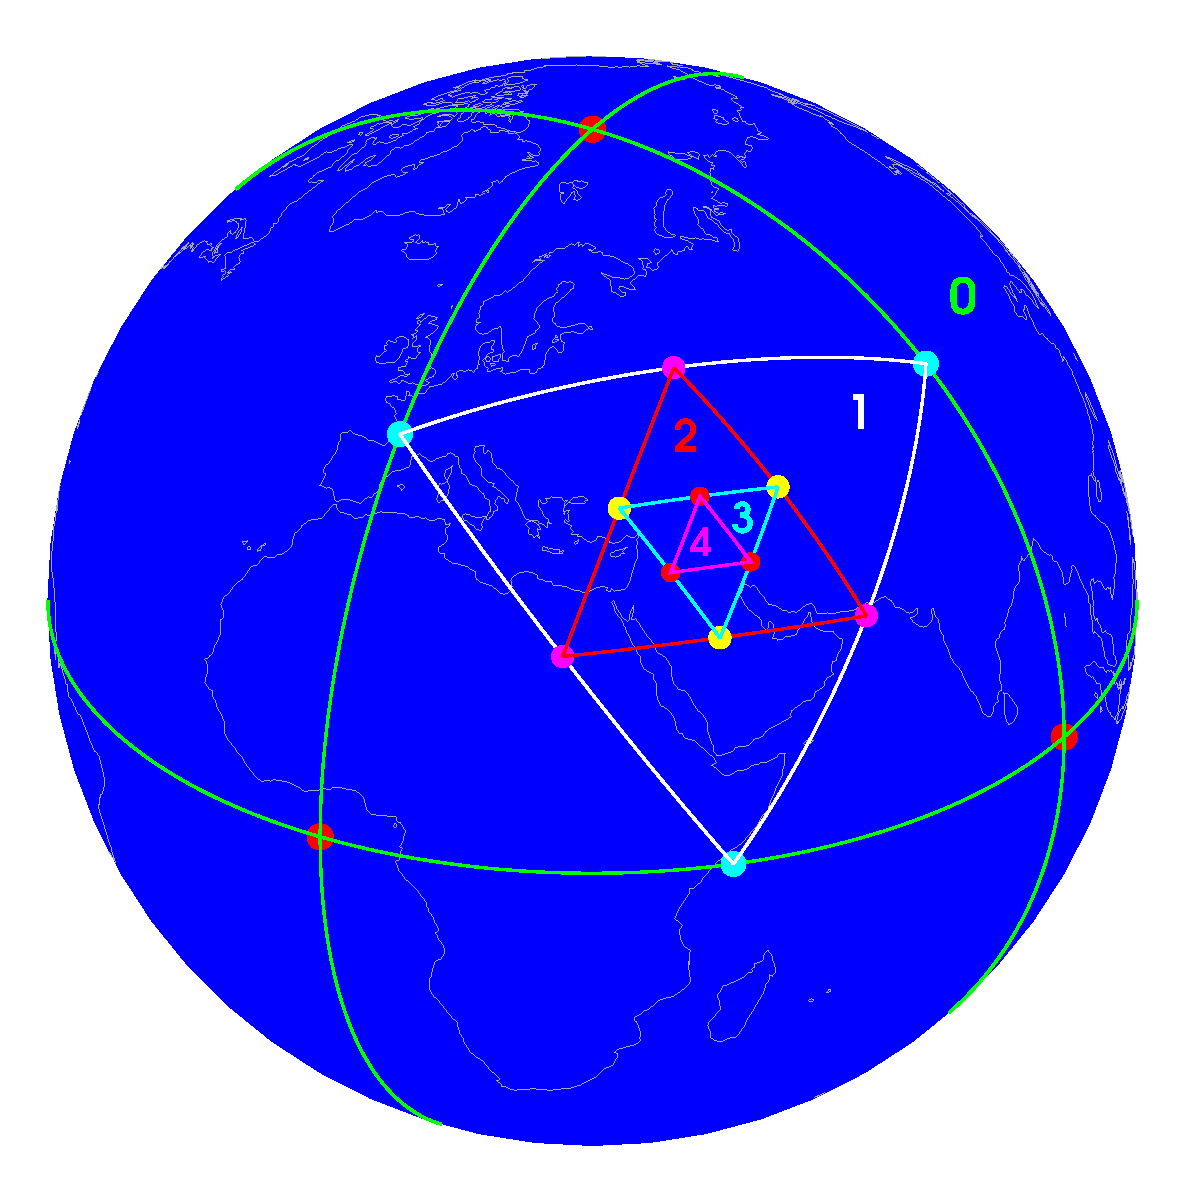
\includegraphics[height=5cm,clip=]{includes/htm_draw_d0-d4}
\caption{(\textit{left}) The 12 HEALPix base pixels color coded for the
 ``ring'' scheme on the plane and the sphere.
 Over-plotted the pixel boundaries for $k=1$ which gives 48 pixels.
 (\textit{right}) The 8 HTM base pixels and recursive subdivisions on
 Earth surface. The ``depth'' $d$ of the trixels is marked.
 }
\label{fig:sphPix}
\end{figure}

%
\subsection{Index choice}
As said, there are two pixelization schema available in \dif: HTM and HEALPix.
Users can choose to use one of them or both. For catalogues and other
general purpose applications, HTM is usually
the best choice because more reliable search criteria are available for not
circular regions.
In order to use \dif\ on a table, the user must provide the following
information to the \texttt{dif} script:
%
\begin{itemize}
\item database name;
\item table name;
\item depth/order of the pixelization scheme:
  \begin{itemize}
    \item HTM, depth $[0:25]$;
    \item HEALPix, resolution parameter: $[0:29]$, for either ordering
      scheme (RING or NESTED, see below);
  \end{itemize}
\item the two field names corresponding to the spherical coordinates (e.g RA
  and Dec, longitude -- $\phi$ and latitude -- $\theta$) \emph{or} a SQL
  compatible expression to compute them.
\end{itemize}
%
\textbf{Note:} starting from Ver. 0.3.3-alpha1 the maximum
resolution parameter for HEALPix is \textbf{29} (it was 13
due to the use of 32 bit integers) corresponding to an angular resolution
of $\sim 4\times 10^{-4}$ arcsec. However, because of 64-bit floating point
arithmetics limitations (e.g. minimum appreciable angular distance),
this limit is not applicable for all the DIF implemented functions.

\textbf{Note:} as Ver. 0.5.4 it is no more required to be root to run
\texttt{dif}. \texttt{dif --grant-user} can be used to grant management permissions
on all tables in a particular DB to a given user.
\bigskip
%

\noindent
The resolution of the pixelization scheme is an important parameter
that will affect the speed at which queries are executed.
Test performed on very large tables have shown that it is not always
true that the greater is the depth the faster will be the query execution.
The query execution time is the result of a number of
operations which depend on several system parameters.
Our results suggest that the most imortant component is the disk seek/access
time and that the CPU usage is a negligible fraction of the total time.
We also found that for tables up to several billion rows, the HTM pixelization
at depth 8 gives the best performance\footnote{L. Nicastro and G. Calderone:
\emph{Multiple depth DB tables indexing on the sphere}, AA, vol. 2010, ID 524534}
(see also \S\ \ref{sec:bench}). This result could be system dependent
but we believe that typically having pixels of size $\sim 20^\prime$ is a
good choice. For large tables this means
that it is adviceble having on average a few thousand entries per pixel.
However the user should make his/her own tests
and choose the most appropriate depth/order. He/she should also consider
if it is worth creating an index on one of the coordinates in conjuction with the
IDs, i.e. for the HTM case, \texttt{htmID-RA}. From our experience,
the use of this two-levels index together with a ``data'' sorting (e.g via
\texttt{myisamchk -R}) could reduce
the query execution time by up to one order of magnitude for very large tables.
Note also that in this case the \dif\ created index
on \texttt{htmID} (only) can be dropped as MySQL/DIF will use the new one
automatically being the pixelization ID the first element of the new
aggregate index. An example is shown in List. \ref{lst_replace_tabindex}.
%
\begin{lstlisting}[
    caption={Example of replacing the default \dif\ index on a table.},
    label={lst_replace_tabindex}]
mysql> DROP INDEX htmID_8 ON MyDB.MyTable;
mysql> CREATE INDEX htmID_8 ON MyDB.MyTable (htmID_8, RA);
\end{lstlisting}

%
\begin{table}[b!]
  \begin{center}
    \caption{Number of pixels and memory requirements associated to
      different levels of resolution parameter for HTM (\emph{depth}\/)
      and HEALPix (\emph{order}\/).}
    \label{tab:depths}
    \footnotesize
    \begin{tabular}{|r|r|r|r|c|}
      \hline
      \multicolumn{1}{|c}{\textbf{Depth/}} &
      \multicolumn{1}{|c|}{\textbf{HTM $N_{\rm pix}$}} &
      \multicolumn{1}{|c|}{\textbf{HEALPix $N_{\rm pix}$}} &
      \textbf{Bytes} & \textbf{Data type}\\
 \multicolumn{1}{|c|}{
       \textbf{Order}} &                   &                       &                &                   \\
      \hline
      $    0 $&$                           8 $&$                             12    $&$         1 $&  TINYINT   \\
      $    1 $&$                          32 $&$                             48    $&$         1 $&  TINYINT   \\
      $    2 $&$                         128 $&$                            192    $&$         1 $&  TINYINT   \\
      $    3 $&$                         512 $&$                            768    $&$         2 $&  SMALLINT  \\
      $    4 $&$                       2,048 $&$                          3,072    $&$         2 $&  SMALLINT  \\
      $    5 $&$                       8,192 $&$                         12,288    $&$         2 $&  SMALLINT  \\
      $    6 $&$                      32,768 $&$                         49,152    $&$         2 $&  SMALLINT  \\
      $    7 $&$                     131,072 $&$                        196,608    $&$         3 $&  MEDIUMINT \\
      $    8 $&$                     524,288 $&$                        786,432    $&$         3 $&  MEDIUMINT \\
      $    9 $&$                   2,097,152 $&$                      3,145,728    $&$         3 $&  MEDIUMINT \\
      $   10 $&$                   8,388,608 $&$                     12,582,912    $&$         3 $&  MEDIUMINT \\
      $   11 $&$                  33,554,432 $&$                     50,331,648    $&$         4 $&  INTEGER   \\
      $   12 $&$                 134,217,728 $&$                    201,326,592    $&$         4 $&  INTEGER   \\
      $   13 $&$                 536,870,912 $&$                    805,306,368    $&$         4 $&  INTEGER   \\
      $   14 $&$               2,147,483,648 $&$                  3,221,225,472    $&$         4 $&  INTEGER   \\
      $   15 $&$               8,589,934,592 $&$                 12,884,901,888    $&$         5 $&  BIGINT    \\
      $   16 $&$              34,359,738,368 $&$                 51,539,607,552    $&$         5 $&  BIGINT    \\
      $   17 $&$             137,438,953,472 $&$                206,158,430,208    $&$         5 $&  BIGINT    \\
      $   18 $&$             549,755,813,888 $&$                824,633,720,832    $&$         5 $&  BIGINT    \\
      $   19 $&$           2,199,023,255,552 $&$              3,298,534,883,328    $&$         6 $&  BIGINT    \\
      $   20 $&$           8,796,093,022,208 $&$             13,194,139,533,312    $&$         6 $&  BIGINT    \\
      $   21 $&$          35,184,372,088,832 $&$             52,776,558,133,248    $&$         6 $&  BIGINT    \\
      $   22 $&$         140,737,488,355,328 $&$            211,106,232,532,992    $&$         6 $&  BIGINT    \\
      $   23 $&$         562,949,953,421,312 $&$            844,424,930,131,968    $&$         7 $&  BIGINT    \\
      $   24 $&$       2,251,799,813,685,250 $&$          3,377,699,720,527,872    $&$         7 $&  BIGINT    \\
      $   25 $&$       9,007,199,254,740,990 $&$         13,510,798,882,111,488    $&$         7 $&  BIGINT    \\
      $   26 $&$                             $&$         54,043,195,528,445,952    $&$         7 $&  BIGINT    \\
      $   27 $&$                             $&$        216,172,782,113,783,808    $&$         8 $&  BIGINT    \\
      $   28 $&$                             $&$        864,691,128,455,135,232    $&$         8 $&  BIGINT    \\
      $   29 $&$                             $&$      3,458,764,513,820,540,928    $&$         8 $&  BIGINT    \\
      \hline
    \end{tabular}
\end{center} \end{table}


%
%
%---------------------------------------------------------------------
\newpage
\section{\dif\ installation}
\label{sec:install}

The \dif\ software library is distributed in a \verb|tar.gz| package.
You can find the latest version at
\url{http://ross.iasfbo.inaf.it/MCS/}. To unpack the package simply
issue the command:
%
\begin{verbatim}
  tar xvzf dif-x.y.z.tar.gz
\end{verbatim}
% 
where \verb|x|, \verb|y|, \verb|z| are the version number (namely
the first number is the major revision, the second number is the
version, and third number is the subversion). A directory named
\verb|dif-x.y.z| will be created containing all the source code as well
as the documentation and the scripts needed to install \dif. Before
installing \dif\ you should check that all the mandatory dependencies are
satisfied (see \S\ \ref{sec:Dependencies}), then you should follow
the procedure described in \S\ \ref{sec:installing}.

\subsection{Dependencies}
\label{sec:Dependencies}
The mandatory packages required by \dif\ are:

\begin{itemize}
\item MySQL (\texttt{http://dev.mysql.com/downloads/}, version 5.1.30 or later) or
\\
 MariaDB (\texttt{https://downloads.mariadb.org/}, version 10.0 or newer) source
 code;
\item Perl (\verb|http://www.perl.com/|);
\item The \verb|DBD::mysql| Perl module;.
\end{itemize}

\noindent
\textbf{Note:} MySQL source code is necessary, not just the
compiled package. The \verb|DBD::mysql| Perl module can be easily
installed through the \verb|cpan| utility issuing the following
command:
%
\begin{verbatim}
  install DBD::mysql
\end{verbatim}
%
See the \verb|cpan| documentation for further information. If these
package are not already installed in the system you should install
them before continuing.
%

\subsection{Installing \dif}
\label{sec:installing}

To install \dif\ you should follow the usual {\tt configure}, {\tt
  make}, {\tt make install} procedures:

\begin{itemize}
\item configuring \dif\ means checking your system for compatibilities,
  search for include files and libraries, and finally produce all
  necessary \textsf{Makefile}s needed to compile the \dif\
  sources. This is done automatically by the distributed
  \verb|configure| script. Typically you should only provide one
  argument to the \verb|configure| script, as follows:
  %
\begin{verbatim}
  ./configure --with-mysql-source=<PATH>
\end{verbatim}
  %
  where \verb|<PATH>| is the absolute path to the MySQL source
  tree. The \verb|configure| script has a lot of options and switches
  (type \verb|configure --help| for a list) to customize the
  compilation step. For further documentation see the \verb|INSTALL|
  file. Nevertheless we recommend not to change the default
  installation path (i.e. the {\tt --prefix=} option).

\item once the \verb|configure| script has been correctly executed
  the compilation of sources is performed with the command:
  %
\begin{verbatim}
  make
\end{verbatim}
  % 
  If you got errors while compiling check the configuration process
  and the \verb|INSTALL| file.

\item once sources are compiled you can install the libraries and the
  scripts with the command:
  %
\begin{verbatim}
  make install
\end{verbatim}
  %
  Usually this command need to be executed as ``root''. In some cases
  it may be helpful to execute the {\tt ldconfig} command (as
  ``root'') to rebuild the shared library cache.

\item finally, to install the DB engine and the \dif\ facilities you
  should issue the command (a running MySQL server is required!):
  %
\begin{verbatim}
  dif --install
\end{verbatim}
  %
  The password of MySQL ``root'' user will be required. Optionally you
  could use the {\tt --log} option to get more information about SQL
  queries being executed.
\end{itemize}
%

\subsection{Upgrade}
\label{sec:upgradedif}
After you have compiled and installed a new version of \dif\ you do not need to issue a
\verb|dif --install| but rather
%
\begin{verbatim}
  dif --upgrade
\end{verbatim}
%
to upgrade UDFs and view definition. In case you are using a very old
version of \dif\ ($\le$ 0.3.3) please contact us and we will try to
help you in this process.
%

Since version 0.5.3, you can eventually use another, partially manual way to
upgrade:
%
\begin{enumerate}
\item open a MySQL session as root and issue these commands:
\begin{verbatim}
  create table test.tbl select * from DIF.tbl;
  delete from DIF.tbl;
\end{verbatim}
  eventually issue similar commands for other tables you may have in \verb|DIF|
  (like \verb|Messier|).
\item uninstall and reinstall \dif:
\begin{verbatim}
  dif --uninstall
  dif --install
\end{verbatim}
  Eventually please see also section \ref{sec:troubles}. In particular after
  the \verb|uninstall| consider restarting the MySQL server.
\item in MySQL restore the \verb|DIF.tbl| table (and eventually more).
\begin{verbatim}
  insert into DIF.tbl select * from test.tbl;
  drop table test.tbl;
\end{verbatim}
  Can view the content of the table, just in case:
\begin{verbatim}
  select * from DIF.tbl;
\end{verbatim}
\end{enumerate}
%
If, for any reason, a \dif\ view was lost or is inconsistent with the content
of \verb|DIF.tbl|, you can recrate it with the option \verb|--views-only| to
\texttt{dif}.
For example let's assume you have installed the Messier catalogue (in DIF, see
section \ref{sec:howitworks}) and want to recreate it:
\begin{verbatim}
  dif --views-only --index-htm DIF Messier 6 Ra Decl
\end{verbatim}
This can be done for any table listed in \verb|DIF.tbl|.

%you need first to deinstall the old version.
%In general this does \textbf{not} mean you need to re-index the tables but
%only execute some shell and MySQL commands. You must have root privileges
%both for MySQL and for the system.
%If you have any trouble please contact us
%and we will try to help you in this process.
%
%Depending on the start version compared to the new one, the upgrade
%process could require either a simple plugin and UDF functions
%re-installation, or, in addition, recreation of all the views, triggers
%and \verb|DIF.dif| and \verb|DIF.tbl| tables.
%In this section users can find all the information required to perform
%the upgrade. In future versions, the upgrade procedure could become
%automatic as an option to the \texttt{dif} command line tool.
%Please note that the upgrade process requires a \textbf{restart} of the
%MySQL server in all cases!
%Open two terminal windows and enter MySQL as user root on one of them
%(e.g. \verb|mysql -u root -p MyCats|, change the DB name to match yours)
%and as system root on the other.
%Here is the procedure.
%
%From version \texttt{0.3.2-alpha3} and \texttt{0.3.3-alpha1}
%  to \texttt{0.5.0}:
%\begin{enumerate}
%\item Get info about indexed tables:
%\begin{verbatim}
%  mysql -u root -p -e "select * from DIF.tbl" > dif_tabs_info.txt
%\end{verbatim}
%give the \texttt{root} password. Output will go into the text file
%\verb|dif_tabs_info.txt|. View its content. It could look like this:
%\small
%\begin{verbatim}
%db   name   HTMDepth   HEALPNested   HEALPOrder   Ra_field   Dec_field
%MyCats   ASCC_25orig    NULL    0      8     RAcs/3.6e5    DECcs/3.6e5
%MyCats   UCAC_2orig     6       0      8     RAcs/3.6e5    DECcs/3.6e5
%\end{verbatim}
%\normalsize
%meaning the catalogue ASCC\_25orig was indexed using HEALPix (RING scheme,
%order 8) and UCAC\_2orig was indexed using HTM (depth 6) and HEALPix
%(RING scheme, order 8). The used fields are RAcs and DECcs (coordinates in
%cent-arcseconds).
%
%\item Drop views (and triggers) for the tables listed in \verb|DIF.tbl|. E.g.:
%\begin{verbatim}
%  dif --drop-view MyCats ASCC_25orig
%  dif --drop-view MyCats UCAC_2orig
%\end{verbatim}
%
%\item Deinstall the old version:
%\begin{verbatim}
%  dif --deinstall
%\end{verbatim}
%Note that starting from version 0.4.0 the option to deinstall is
%\verb|--uninstall| so be sure you execute this command with the
%currently installed (\emph{old}) version!
%Also note that in version 0.3.2-alpha3 this operation will not check the
%tables status, i.e. indexes and DIF created columns will not be touched.
%
%\item Compile and install the new version as described in the previous sections.
%  If you get any error, please contact us.
%
%\item From the shell terminal stop the MySQL server:
%\begin{verbatim}
%  /etc/init.d/mysql.server stop
%\end{verbatim}
%or whatever command your system requires.
%
%\item Reinstall \dif\ as described in the previous section and restart the
%MySQL server (the \verb|ldconfig| is to
%force the system to read the changed \verb|ha_dif.so| file):
%\begin{verbatim}
%  ldconfig
%  /etc/init.d/mysql.server start
%  dif --install
%  /etc/init.d/mysql.server restart
%\end{verbatim}
%If you get any error, please check section \ref{sec:troubles}. If that
%does not help, contact us.
%
%\item[6a.] Update (index) columns names to match new defaults.
%\begin{framed}
% \textbf{Note:} it is preferable that also the \emph{default value} is
%  reset from \verb|NULL| to 0, but this operation could take some time to be
%  performed on large tables. If you choose to do so, please see next point.
%\end{framed}
%In the MySQL session give (this is for one of the tables of the example above):
%\begin{verbatim}
% alter table MyCats.UCAC_2orig change htmID htmID_6 smallint unsigned;
% alter table MyCats.UCAC_2orig change healpID healpID_ring_8 smallint
%   unsigned;
%\end{verbatim}
%Be sure you keep column(s) type(s) the same!
%Column types can be viewed using e.g.
%\verb|describe MyDB.MyTable|.
%For a table using HEALPix NESTED scheme ``\verb|ring|'' becomes ``\verb|nest|''.
%\\
%\rule{6cm}{1pt}
%
%\item[6b.] Update (index) columns names \emph{and} default values to match new defaults.
%\begin{framed}
% \textbf{Note:} This is an alternative to the previous step and it is not
% compulsory. It could take some time to execute because index files must be
% recreated, still it is
% preferable to perform it. You can decide to perform it at a later time,
% e.g. running the command(s) overnight.
%\end{framed}
%In the MySQL session give (this is for one of the tables of the example above):
%\begin{verbatim}
% lock tables MyCats.UCAC_2orig write;
% alter table MyCats.UCAC_2orig disable keys;
% alter table MyCats.UCAC_2orig change htmID htmID_6 smallint unsigned
%   not null default 0;
% alter table MyCats.UCAC_2orig change healpID healpID_ring_8 smallint
%   unsigned not null default 0;
% alter table MyCats.UCAC_2orig enable keys;
% unlock tables;
%\end{verbatim}
%
%%
%%An apparently more complex but actually faster way is the following
%%(it only applies to MyISAM tables):
%%\begin{enumerate}
%%%
%%\item in the shell terminal go into the directory coresponding to the
%% database \verb|MyCats|, e.g. \verb|cd /usr/local/mysql/var/MyCats|;
%%\item for each DIF protected table backup the \verb|.frm| file, for example \\
%% \verb|cp UCAC_2orig.frm UCAC_2orig.frm_old|;
%%\item for each table, in the MySQL session:
%%  \begin{itemize}
%%  \item create a table with the identical schema to the one you want to alter
%%   and perform the changes on this table, for example for \verb|UCAC_2orig|:
%%\small
%%\begin{verbatim}
%% create table t1 like UCAC_2orig;
%% drop index htmID on t1; drop index healpID on t1;
%% alter table t1 change htmID htmID_6 smallint unsigned not null
%%   default 0;
%% alter table t1 change healpID healpID_ring_8 smallint unsigned
%%   not null default 0;
%% create index htmID_6 on t1 (htmID_6);
%% create index healpID_ring_8 on t1 (healpID_ring_8);
%%\end{verbatim}
%%\normalsize
%%Be sure you keep column type the same!
%%Now if you have any ``suspect'' that \verb|NULL| values are present in your
%%table(s), execute the following commands, too:
%%%
%%\small
%%\begin{verbatim}
%% update UCAC_2orig set htmID=0 where isnull(htmID);
%% update UCAC_2orig set healpID=0 where isnull(healpID);
%%\end{verbatim}
%%%
%%\normalsize
%%This operation will be fast as it uses indexed columns.
%%After you have finished with all the tables (of course for
%%  each of them change \verb|t1| into something else):
%%  \item stop the MySQL server;
%%%  \item from the shell terminal overwrite the original \verb|.frm|
%%%  with the newly created, e.g. \verb|cp t1.frm UCAC_2orig.frm|;
%%  \item move (or copy, if dont't have and want to keep a backup) the data
%%  file: \verb|mv UCAC_2orig.MYD t1.MYD| and rename the index file: \\
%%  \verb|mv UCAC_2orig.MYI UCAC_2orig.MYI_old| (you'll remove it later);
%%  \item restart the MySQL server:
%%  \item in the MySQL shell give the commands:\\
%%  \verb|repair table t1;| \\
%%  \verb|rename table t1 to UCAC_2orig;| \\
%%  The repairing is to update the number of rows in the index file.
%%  It can be done using \verb|myisamchk -r| before restarting the server.
%%  \item  to see that all is ok give, e.g., the commands: \\
%%  \verb|show table status like 'UCAC_2orig';| \\
%%  \verb|show index from UCAC_2orig;|
%%  \end{itemize}
%%%
%%%
%%\end{enumerate}
%%
%As you can see, the commands change names and default value for the index
%column(s). It was \verb|NULL| whereas now it is 0.
%This is to avoid unnecessary checks for undefined column
%values to the MySQL server.
%As above, be sure you keep column(s) type(s) the same!
%For a table using HEALPix NESTED scheme ``\verb|ring|'' becomes ``\verb|nest|''.
%\\
%\rule{6cm}{1pt}
%
%\item Recreate views (and triggers) for the tables above, e.g.:
%\begin{verbatim}
%  dif --index-views MyCats ASCC_2orig
%  dif --single-index-views MyCats UCAC_2orig
%\end{verbatim}
%ignore any warning message...
%%
%\end{enumerate}
%%
%\emph{For older versions please contact us}!

%---------------------------------------------------------------------
%\newpage
%\section{How it works}
%In this section we present the detailed mechanism on which \dif\
%relay. Several tasks described here are automatically performed by
%\dif\ so users not interested in this subject may skip to next section.
%
%\bigskip
%
%In a typical astronomical application there is a catalogue stored on a
%database table, in which each entry is a single object with its own
%coordinates (see List. \ref{lst_messier}). \dif\ adds one (or more)
%column(s) to the table to associate an HTM (and/or a HEALPix) ID to
%each entry (last column in List. \ref{lst_messier}), and creates a
%database index on it to take advantage of the MySQL indexing
%system. This way we ensure maximum speed allowed by MySQL in queries
%execution.
%%
%\begin{lstlisting}[
%    caption={Example of an astronomical catalogue.},
%    label={lst_messier}]
%mysql> SELECT * FROM Messier;
%+-----+------+-------+------+---------+------------+------------+---------+
%| M   | Type | Const | Mag  | Ra      | Decl       | Dist       | htmID_6 |
%+-----+------+-------+------+---------+------------+------------+---------+
%|   1 | BN   | Tau   |  8.2 |  83.625 |    22.0167 | 6.3 kly    |   62340 |
%|   2 | GC   | Aqu   |  6.3 | 323.375 |  -0.816667 | 36.2 kly   |   47406 |
%|   3 | GC   | CVn   |  6.3 | 205.549 |    28.3833 | 30.6 kly   |   56399 |
%|   4 | GC   | Sco   |  6.4 | 245.876 |    -25.475 | 6.8 kly    |   43651 |
%|   5 | GC   | Ser   |  6.2 |  229.65 |    2.08333 | 22.8 kly   |   53765 |
%....
%\end{lstlisting}
%% 
%On the other hand \dif\ provides a list of HTM (and/or a HEALPix) IDs
%matching a search criteria through the {\tt DIF.dif} table (see
%List. \ref{lst_example_dif}).
%%
%\begin{lstlisting}[
%    caption={Specifying a search criteria using \dif.},
%    label={lst_example_dif}]
%mysql> SELECT DIF_setHTMDepth(6);              #Use HTM depth 6
%mysql> SELECT DIF_HTMCircle(83.6, 22, 100);    #Search criteria: circle centered
%                                               #in RA=83.6, Dec=22 with radius=100
%mysql> SELECT * FROM DIF.dif;                  #Dynamical content of table DIF.dif
%+-------+-------+------+
%| param | id    | full |
%+-------+-------+------+
%|     6 | 62392 |    1 |
%|     6 | 61832 |    0 |
%|     6 | 61860 |    0 |
%|     6 | 61876 |    0 |
%|     6 | 62340 |    0 |
%|     6 | 62341 |    0 |
%|     6 | 62342 |    0 |
%|     6 | 62343 |    0 |
%|     6 | 62348 |    0 |
%|     6 | 62350 |    0 |
%|     6 | 62351 |    0 |
%|     6 | 62360 |    0 |
%|     6 | 62362 |    0 |
%|     6 | 62363 |    0 |
%|     6 | 62393 |    0 |
%|     6 | 62394 |    0 |
%|     6 | 62395 |    0 |
%+-------+-------+------+
%\end{lstlisting}
%%
%The contents of the {\tt DIF.dif} table are dynamically generated
%following the specified search criteria, thus the {\tt DIF.dif} table
%does not store any data on disk. The available fields are:
%%
%\begin{itemize}
%\item {\tt param}: HTM depth/HEALPix order;
%\item {\tt id}: HTM/HEALPix pixel ID;
%\item {\tt full}: whether the HTM/HEALPix pixel is entirely contained
%  in the specified search region; 
%\end{itemize}
%%
%Finally \dif\ perform a join between the catalogue table and the {\tt
%  DIF.dif} table to select only the desired records (see
%List. \ref{lst_example_dif2}).
%%
%\begin{lstlisting}[
%    caption={Join of catalogue table and {\tt DIF.dif} table.},
%    label={lst_example_dif2}]
%mysql> SELECT Messier.* 
%       FROM DIF.dif JOIN Messier 
%       ON ((Messier.htmID_6 = DIF.dif.id) AND (DIF.dif.param = 6));
%+---+------+-------+------+--------+---------+---------+----------+---------+
%| M | Type | Const | Mag  | Ra     | Decl    | Dist    | App_size | htmID_6 |
%+---+------+-------+------+--------+---------+---------+----------+---------+
%| 1 | BN   | Tau   |  8.2 | 83.625 | 22.0167 | 6.3 kly | 6'x4'    |   62340 |
%+---+------+-------+------+--------+---------+---------+----------+---------+
%\end{lstlisting}
%%
%

%\newpage
\section{How \dif\ works}
\label{sec:howitworks}
Consider an astronomical catalog stored on a database table in which
each entry has two fields in which the coordinates of a
latitude/longitude system are stored. The \dif\ approach is to split
the sphere into a finite number of zones (or ``pixels'') and associate
an ID to each of these pixels. The association is based on one of the
pixelization schemas described in \S\ \ref{sec:pixschema}. Thus a
pixel ID can be associated to each entry in the table. \dif\ will add a
field to the table to store such IDs and creates an index on it,
relaying on the built-in MySQL indexing system. Then \dif\ provides a
way to dynamically generate a list of pixel IDs corresponding to a
given search criteria, and perform a SQL join between the indexed
table and the pixel list, thus providing very fast query execution.
The pixel ID list is provided through the {\tt DIF.dif} table; this is
not a usual table since it does not occupy any space on the disk, its
content is dynamically generated based on the user specified search
criteria. This functionality is provided by the \dif\ DB engine. The
generation of the pixel ID list and the SQL join are completely
transparent to the user once the \dif\ views are used to access the
table.
%

In the following example we will refer to the {\tt Messier} table
which is automatically installed in the {\tt DIF} database during \dif\
installation. Other astronomical tables with many more entries can be
downloaded from \url{http://ross.iasfbo.inaf.it/MCS/}.
The \verb|Messier| table has the following structure:
%
\begin{lstlisting}[
    caption={Structure of the {\tt Messier} table.},
    label={lst_messier_struct}]
mysql> describe Messier;
+----------+----------------------+------+-----+---------+-------+
| Field    | Type                 | Null | Key | Default | Extra |
+----------+----------------------+------+-----+---------+-------+
| M        | int(11)              | NO   |     | NULL    |       |
| Type     | char(2)              | YES  |     | **      |       |
| Const    | char(3)              | YES  |     | ***     |       |
| Mag      | float                | YES  |     | NULL    |       |
| Ra       | float                | YES  |     | NULL    |       |
| Decl     | float                | YES  |     | NULL    |       |
| Dist     | char(20)             | YES  |     | NULL    |       |
| App_size | char(20)             | YES  |     | unknown |       |
+----------+----------------------+------+-----+---------+-------+
\end{lstlisting}
The equatorial coordinates in degrees of each object is stored in the
{\tt Ra} and {\tt Decl} fields. Any other coordinate system can be
used as well, provided it can be transformed to a latitude
($[-90:90]$) / longitude ($[0:360]$) spherical system. To use the
\dif\ indexing system upon this table we should issue a command like:
%
\begin{verbatim}
  dif --index-htm DIF Messier 6 Ra Decl
\end{verbatim}
%
In this case the HTM pixelization scheme with depth 6 is used. Note
that we passed the name of the fields containing the coordinates in
the command line. The {\tt dif} script will:
%
\begin{itemize}
\item add a new field named {\tt htmID\_6} (of type {\tt smallint}) to
  the table and populate it with the HTM ID corresponding to the
  coordinates of the object;
\item create an index on {\tt htmID\_6};
\item create a view named {\tt Messier\_htm\_6} which trasparently
  perform the join between the {\tt Messier} and {\tt DIF.dif} table;
\item define triggers so that the {\tt htmID\_6} field will be
  automatically populated with the correct HTM ID each time the {\tt
    Messier} table is modified.
\end{itemize}
Now the user can access the indexed table through the {\tt
Messier\_htm\_6} view. The search criteria are specified in the {\tt
SELECT} query using the {\tt DIF\_Circle} (or another
region-defining) function\footnote{Note that from Ver. 0.5.2 the prefix
{\tt HTM/HEALP} has been removed from these functions as the pixelization
scheme is derived directly from the view used}, as in the example shown in
List. \ref{lst_queryexample}
\begin{lstlisting}[
    caption={Example query on the Messier table.},
    label={lst_queryexample}]
mysql> SELECT * FROM Messier_htm_6 WHERE DIF_Circle(82, 22, 100);
+---+------+-------+------+--------+---------+---------+---------+-----------+--------+
| M | Type | Const | Mag  | Ra     | Decl    | Dist    | htmID_6 | HTM_Depth |HTM_Full|
+---+------+-------+------+--------+---------+---------+---------+-----------+--------+
| 1 | BN   | Tau   |  8.2 | 83.625 | 22.0167 | 6.3 kly |   62340 |         6 |       0|
+---+------+-------+------+--------+---------+---------+---------+-----------+--------+
1 row in set (0.00 sec)
\end{lstlisting}
Although the table used in the example has only 110 records, the
notable aspect here is that with \dif\ the same query can be executed
even on a table with several billions records and the execution time
will be approximately the same for any table, provided the index has
been chosen carefully (see \S\ \ref{sec:bench}). A schematic view of
the entire process is show in Fig. \ref{fig:schemadif}.
%
\begin{figure}[hbtp]
\begin{center}
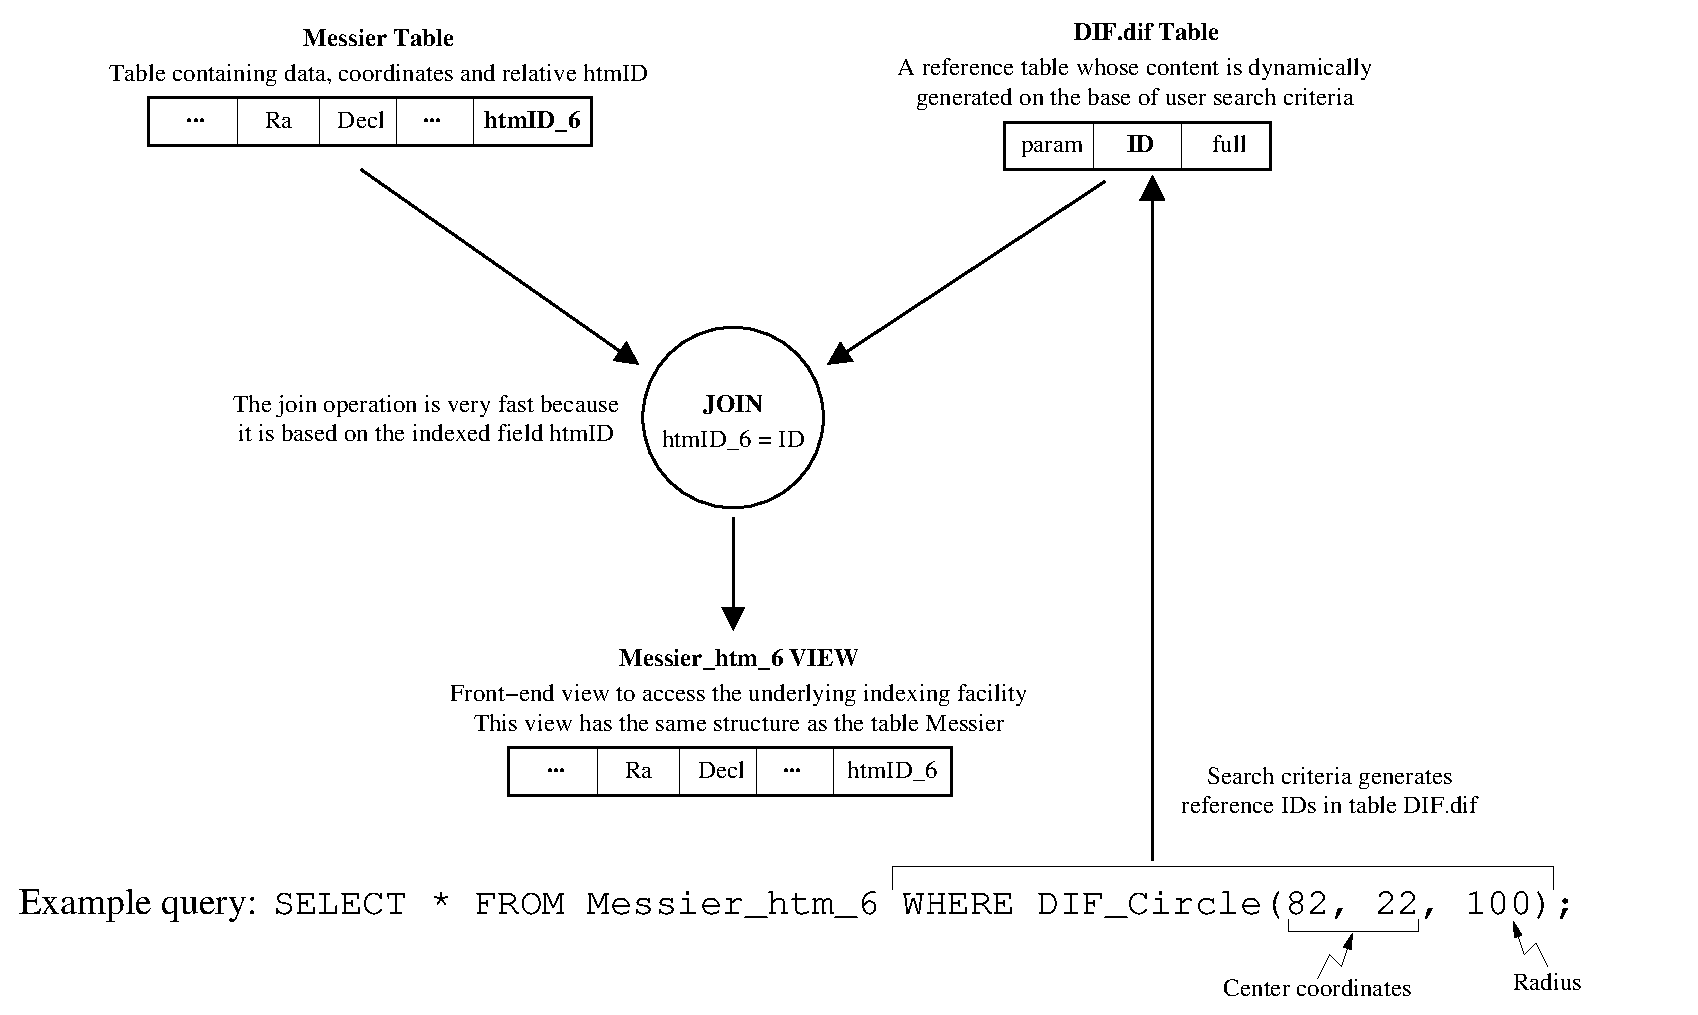
\includegraphics[width=14cm,keepaspectratio]{includes/schema}
\end{center}
\caption{Schematic view of the tables involved in a \dif\ query.}
\label{fig:schemadif}
\end{figure}
%
In many cases using one single index would suffice all the user's needs.
However any number and type of \dif\ indices can be added to the table.
Depending on the system requirements, this could positively affect the
overall performance.
How many and which type of indices one should use, typically depends on the
number of entries in the table and the (range of) size of the sky regions
queried. We will discuss this below, but we also recommend to read the
reference paper ``\emph{Nicastro and Calderone, AA, vol. 2010, ID 524534}''.
Thus a user may want, e.g., to add
also a HTM index of depth 8 and an HEALPix nested index of order 10;
this is easily done with the command:
\begin{verbatim}
  dif --index-htm DIF Messier 8 Ra Decl \
      --index-healpix-nested DIF Messier 10 Ra Decl
\end{verbatim}
Because an additional HTM depth is present, an ``aggregate'' view
{\tt Messier\_htm} will be created.
Users should perform the query on the view corresponding to the index
to be used, in this case {\tt Messier\_htm\_6}, {\tt Messier\_htm\_8} or {\tt
Messier\_healp\_nest\_10}. Optionally, to use simultaneously the two
HTM indices 6 and 8, one can query the view {\tt Messier\_htm}.
It uses {\tt UNION ALL} statements to perform the query on all the
available depths and return a single list of entries. Note, however, that
\dif\ performs a single call to the HTM routine to get the
list of IDs at the various depths by performing a ``recursive erosion''
of the queried region (see the above cited reference paper). These IDs are
then used to feed the {\tt DIF.dif} table as in the single depth case
(see below).

%
\subsection{The search criteria}
The search criteria used to dynamically populate the {\tt DIF.dif}
table are specified through one of the following functions:
\begin{itemize}
\item {\tt DIF\_Circle}: circle (cone) region;
\item {\tt DIF\_Rect}: rectangular region giving sides;
\item {\tt DIF\_Rectv}: rectangular region giving vertices;
\item {\tt DIF\_NeighbC}: region of a central pixel and its neighbors.
\item {\tt DIF\_sNeighb}: region of neighbors at higher depth (smaller pixel) around
a central pixel. \emph{Only implemented for HTM pixelization.} See e.g. Fig. \ref{fig:htmsneighb}.
\end{itemize}
\textbf{Note:} starting from Ver. 0.5.2 the prefix {\tt HTM/HEALP}, used to
identify the functions that apply to the two types of pixelizations, have
been dropped. In fact these functions now inherit the information on the
pixelization directly from the views they apply to.
The parameters of such functions are described in
\S\ \ref{sec:DIF_function_reference}. \dif\ will remember search
criteria between successive queries until a new search criteria is
specified. Thus, assuming these indices exist, the following queries will
return exactly the same set of records:
\begin{verbatim}
  SELECT * FROM Messier_htm_6 WHERE DIF_Circle(82, 22, 100);
  SELECT * FROM Messier_htm_8;
  SELECT * FROM Messier_htm;
  SELECT * FROM Messier_healp_nest_10;
\end{verbatim}
Indeed the only difference may be in the queries execution times since
different indexes could provide different performance. Furthermore, search
criteria may be specified before accessing the view, as in the
following example:
\begin{verbatim}
  SELECT DIF_Circle(82, 22, 100);
  SELECT * FROM Messier_htm_6;
\end{verbatim}
%
\textbf{Note:} future versions of
\dif\ will eventually allow combining (through logical AND and OR) different
regions. However this will require to drop the creation (and then availability)
of the aggregate view ({\tt \_htm}). We then suggest to use in the queries
only the depth specific views to avoid the need to change program and scripts
code in the future.
%
% ./htmsNeighbMylookup 6 64575 10 > fig_htms.out
% htm_plot, 'fig_htms.out',ra=11.,de=44.,side=4.5,/enc,/ps
\begin{figure}[hbtp]
\begin{center}
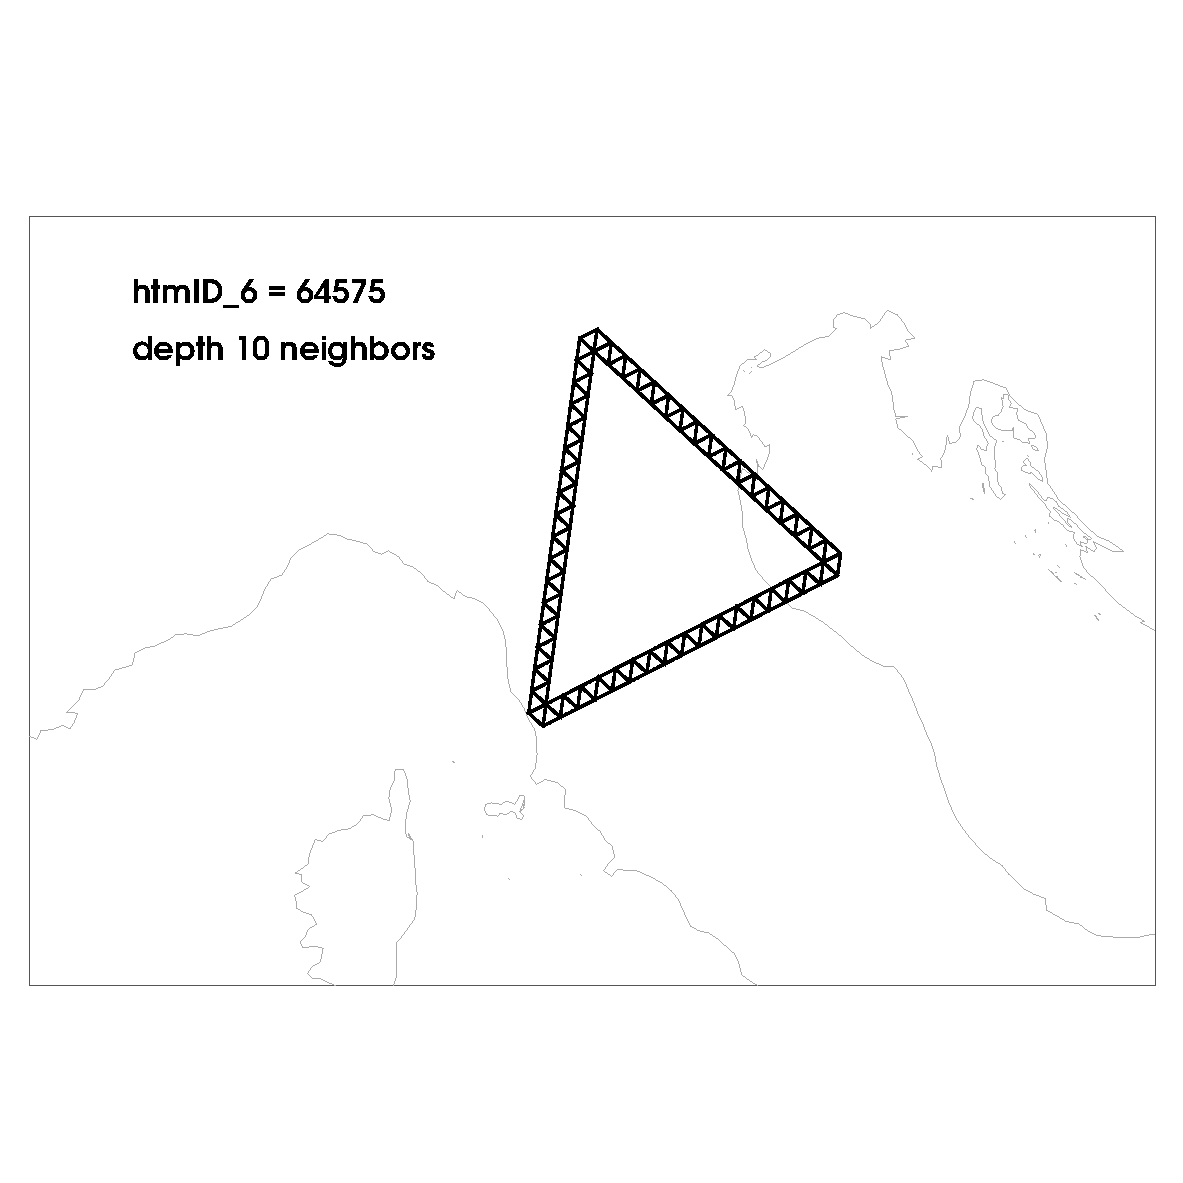
\includegraphics[trim=1.5cm 4cm 1.5cm 4cm, width=14cm, clip,keepaspectratio]{includes/htm6-10neighb_plot}
\end{center}
\caption{Earth view of the HTM depth 10 neighbors to the depth 6 trixel with
ID 64575 (covering Bologna $[lon,lat] \simeq [11,44]$). This selection can
be done via the UDF function \texttt{HTMsNeighb} or via \texttt{DIF\_sNeighb}
in a \dif\ query (see below).}
\label{fig:htmsneighb}
\end{figure}

\subsection{\texttt{DIF.tbl} and \texttt{DIF.func} tables}
The {\tt DIF.tbl} table is used to store the basic information about the
tables being handled by \dif.
Its structure is shown in List. \ref{lst_tbl_struct}.
\begin{lstlisting}[
    caption={Structure of the {\tt DIF.tbl} table.},
    label={lst_tbl_struct}]
mysql> describe DIF.tbl;
+-----------+--------------+------+-----+---------+-------+
| Field     | Type         | Null | Key | Default | Extra |
+-----------+--------------+------+-----+---------+-------+
| db        | varchar(64)  | YES  | MUL | NULL    |       |
| name      | varchar(128) | YES  |     | NULL    |       |
| id_type   | int(11)      | NO   |     | NULL    |       |
| id_opt    | int(11)      | NO   |     | 0       |       |
| param     | int(11)      | NO   |     | NULL    |       |
| Ra_field  | varchar(128) | YES  |     | NULL    |       |
| Dec_field | varchar(128) | YES  |     | NULL    |       |
+-----------+--------------+------+-----+---------+-------+
\end{lstlisting}
\textbf{Note:} the string (\texttt{varchar}) fields were extended in v. 0.5.4.

\medskip
The {\tt DIF.func} table is used to store information about \dif\ functions
and procedures. It is used by the \texttt{difInfo} SQL procedure.
Its structure is shown in List. \ref{lst_func_struct}.
\begin{lstlisting}[
    caption={Structure of the {\tt DIF.func} table.},
    label={lst_func_struct}]
mysql> describe DIF.func;
+-------------+------------------------------------------+------+-----+-----------+
| Field       | Type                                     | Null | Key | Default   |
+-------------+------------------------------------------+------+-----+-----------+
| name        | char(64)                                 | YES  |     | unknown   |
| params      | varchar(128)                             | YES  |     | undefined |
| ret         | char(16)                                 | YES  |     | string    |
| type        | enum('function','procedure','aggregate') | YES  |     | NULL      |
| plugin_lib  | char(64)                                 | YES  |     |           |
| description | varchar(256)                             | YES  |     |           |
+-------------+------------------------------------------+------+-----+-----------+
\end{lstlisting}
\textbf{Note:} this table was added in v. 0.5.4.

\subsection{Structure of the \texttt{DIF.dif} table}
The {\tt DIF.dif} table is the core of the \dif\ since it provides the
(either HTM or HEALpix) pixel list IDs against which indexed table are
to be joined, based on user search criteria. It also reports if a
given pixel is fully or partially included in the requested
region. The \texttt{dif} table is based on the \dif\ database engine,
thus it is different from other database tables since it doesn't
occupy any space on disk but its content is dynamically generated
using the \dif\ functions. Also the table content is different for each
MySQL connection, that is a user cannot see the content of the
\texttt{dif} table of another user. 
%The content of the table only
%exists at query time. It can be though as a Linux ``pipe'' file which
%only returns data if a process is writing into it.  The functions that
%can be used to generate the content of the \texttt{dif} table are (see
%\S\ \ref{sec:DIF_function_reference}):
%%
%\begin{center}
%\begin{tabbing}
% \verb|DIF_HTMNeighbC|~~ \= ~~\verb|DIF_HEALPCircle|~~ \= ~~\verb|DIF_HTMRectV|~~ \= ~~ \kill
% \verb|DIF_HTMCircle| \> \verb|DIF_HTMRect| \> \verb|DIF_HTMRectV| \>
%   \verb|DIF_HTMNeighbC| \\
% \verb|DIF_HEALPCircle| \> \verb|DIF_HEALPNeighbC| \> ~~ \>
%\end{tabbing}
%\end{center}
%%
%Each of these functions provides a way to select entries falling into
%different kinds of
%region on a sphere or to define a list of neighbors IDs.
%The \verb|Circle| and \verb|Rect| region selecting functions transparently
%use the DB engine function \verb|DIF_FineSearch| which will filter
%out the entries falling in the partially covered pixels which are not
%within the requested area.
%As the list suggests, the HTM library allows us to implement and add more
%functions than the HEALPix library. This is because it was specifically
%designed to perform region
%selections and indexing. Still other functions are
%planned to be added in future versions for both pixelizations.
The structure of the \texttt{dif} table is show in
List. \ref{lst_dif_struct}.
\begin{lstlisting}[
    caption={Structure of the {\tt DIF.dif} table.},
    label={lst_dif_struct}]
 mysql> describe DIF.dif;
 +-------+------------+------+-----+---------+-------+
 | Field | Type       | Null | Key | Default | Extra |
 +-------+------------+------+-----+---------+-------+
 | param | int(11)    | YES  |     | NULL    |       |
 | id    | bigint(20) | YES  |     | NULL    |       | 
 | full  | tinyint(1) | YES  |     | NULL    |       | 
 +-------+------------+------+-----+---------+-------+
\end{lstlisting}
The first field, \verb|param|, gives the depth (HTM) or order
(HEALPix) of the pixelization, the second contains the pixel ID and
the third is a flag indicating if the pixel is entirely included (1)
or partially included (0) in the user selected region. The
\texttt{dif} table should never be used directly, instead user should
use one of the views provided by \dif. The name of these views is made
up of the name of the indexed table and a suffix that depends on the
type of index (either \verb|_htm|, \verb|_healp_nest| or
\verb|_healp_ring|) followed by an integer which represents the
depth/order.  The structure of these views is exactly the same as the
data table on which they are based.


%%
%\subsection{Views}
%\label{sec:views}
%Select queries on sky regions are performed via ``joins'' between the indexed
%table and the \verb|DIF.dif| dynamic table. There are two ways to instruct
%\dif\ to perform queries on a given region: using a view specific
%for a particular
%depth/order or using all the available indexes (HTM or HEALPix -- ring or
%nested) at once. For a table \verb|MyTab| managed by DIF, the main view
%\verb|MyTab_htm| and/or \verb|MyTab_healp| are created.
%Those views can be used to query the table using all the available indexes.
%Alternatively views referring to each index, i.e. pixelization type
%and size, can be created and used. In this case the views will be of the type
%\verb|MyTab_htm_8| or \verb|MyTab_healp_nest_8| (see below).
%
%
%
%), thus containing some fields with the coordinate
%of an object. Any coordinate system can be used, provided it an be
%transformed to a latitude ($[-90:90]$) / longitude ($[0:360]$)
%spherical system. Once installed, \dif\ will add a new field to the
%table containing the HTM (and/or HEALPix) ID of the pixel in which the
%coordinates are located, and a database index upon this field that
%will allow fast execution of queries. Direct use of this index in
%queries is nevertheless not easy, so \dif\ provides a set of tools
%aimed at using the index in an effective trasparent way. The main
%component of a \dif\ system is a database engine, that is a pluggable
%MySQL module able to present dynamic data as if they were stored into
%a conventional database table (the \texttt{DIF.dif} table). Actually
%data coming from the \dif\ engine are the HTM (or HEALPix) IDs of the
%pixels that match the user search criteria. Considering that this data
%are seen as a conventional table it is possible to perform a join
%between the \texttt{MAIN} table and the \texttt{dif} table, thus
%locating the records very quickly. Other components of the \dif\ system
%are: 1. SQL and SQL callable external C++ functions, 2. DB engine
%specific functions (also written in C++), 3. views and triggers that
%allow a trasparent use of the underlying indexing system. All the
%functions related to the pixelizations rely on the corresponding HTM
%and HEALPix C++ libraries (see http://www.sdss.jhu.edu/htm/ and
%http://healpix.jpl.nasa.gov/).
%
%\bigskip
%In a typical astronomical application there is the need to select all the
%objects located inside a certain region of the sky (see Fig.
%\ref{fig:schemadif}). As already explained, there are two tables
%involved, the \texttt{MAIN} table and the \texttt{dif} table, which
%are joined, e.g., on the \verb|htmID| field. Tables can also be joined
%using the HEALPix scheme in a completely analogous way (both the RING
%or NESTED map ordering can be used). Data are seen through a view that
%hides all the join and \dif\ mechanisms. The search criteria are specified
%in the WHERE clause of the query through the use of a \dif\ function
%and its parameters, as can be seen in the query at the bottom of Fig.
%\ref{fig:schemadif}. In this case the \verb|DIF_HTMCircle| will select
%a circular region centered at coordinates $10^\circ$, $20^\circ$ and
%with a radius of $3'$. The content of the \texttt{dif} table is
%dynamically generated on the base of the user search criteria
%specified through the \dif\ functions. \\
%Note: starting from version 0.5.0, the region
%selection criteria can be invoked once and then used in subsequent
%select queries as many times as the user wants. In other words \dif\ keeps
%memory of the last requested region and implicitly performs all the
%queries on the sub-set of rows intercepted by that region until a new
%region is specified. Moreover the user can choose if only one or all the
%available indexes should be used for the query. These issues are
%discussed in some details below, but we anticipate that it is good
%practice to perform tests and benchmarks in order to identify
%the best choices for a given table and system in use.




%---------------------------------------------------------------------
\newpage
\section{\dif\ usage}
\label{sec:usage}
All administrative tasks related to \dif\, like creating or dropping
indexes and views, can be accomplished using the \verb|dif|
script. All available options and commands can be displayed using the command:
%
\begin{verbatim}
  dif --help
\end{verbatim}
%
The {\tt dif} script (written in Perl) has options and commands,
the former are used to enable a specific facility (logging, interactive
interface, etc.) while the latter are used to accomplish administrative
tasks. Each command requires its arguments which may be given on the
command line or inserted interactively upon request from the
script. Any number of options and commands (eventually followed by
arguments) can be given on a single command line. Options must be
given before commands. The {\tt dif} script always requires the MySQL
``root'' password unless a user was granted admin permissions on a given DB
tables using the command \texttt{dif --grant-user}.

\subsection{{\tt dif} options}
As version 0.5.4, available options are (for current list see \verb|dif -h|):
%
\begin{verbatim}
-h | --help     print this usage message.
-v | --ver      print version number.
--interactive   use interactive interface.
--log           print SQL queries on standard output.
--logfile       print SQL queries on file dif.sql.
--multidx       create or update the multi-index view for HTM (Tab_htm).
--trigger       add or update the INSERT trigger for input table.
--no-multidx    do not create/update the multi-index view for HTM (Tab_htm). Def.
--no-trigger    do not add/update the INSERT trigger for input table. Def.
--views-only    recreate all the table views and trigger but do not touch table
                and indices. Must preceed --index-htm or --index-healpix-xxx comm.
--readonly      do not execute any query that would modify the database.
--cnf           read user and/or password from "~/.my.cnf".
--ra-key        add RA field to the index (i.e. ID+RA, def. ID only).

-u | --user <User>
                Perform operations below as User rather than as root.
                Assume that root granted User the required privileges for
                view creation and INSERT/DELETE operations on DIF.tbl.

-p | --pass <Password>
                root or User password.
\end{verbatim}
%
Again, these must be given before any command.
There can be any number of commands, each followed by its own
arguments. When using the interactive interface the arguments must be
given through stdin and those on command line will be ignored.

Notes (since Ver. 0.5.4 these options are the default):
\begin{itemize}
\item if your table is only used in read mode (\verb|SELECT|) or you'll take
 care to compute on the fly the HTM/HEALPix IDs via \verb|HTMLookup| or
 \verb|HEALPLookup| \dif\ functions, then you can use the option
 \verb|--no-trigger| to avoid the creation of the triggers for \verb|INSERT|
 queries; 
\item if you are not a specialized user, then it's likely that you will
 index the table using one HTM depth. Or eventually you'll index on various depths
 but you are not going to take advantage of multiple HTM depths capability.
 In these cases it is better you use the \verb|--no-multidx| to avoid creating
 the aggregate \verb|XYZ_htm| table.
%
\end{itemize}

If the user/password are read from the \texttt{~/.my.cnf} configuration file,
they are read from the first section present. An example file is:
\begin{verbatim}
[client]
user = testusr
password = testpasswd
host = localhost
\end{verbatim}

%
\subsection{Indexing a table using \dif}
To index a table using \dif\ you should execute the {\tt dif} script
with one or more of the following commands:
%
\begin{itemize}
\item {\tt --index-htm <DBName> <Table> <Depth> <Ra\_deg> <Dec\_deg>};
\item {\tt --index-healpix-ring  <DBName> <Table> <Order> <Ra\_deg> <Dec\_deg>};
\item {\tt --index-healpix-nested  <DBName> <Table> <Order> <Ra\_deg> <Dec\_deg>};
%
\end{itemize}
The first will add an index using the HTM pixelization scheme with the
desired depth, the last two will use the HEALPix (respectively with
RING and NESTED) scheme of desired order. Arguments meaning are:
%
\begin{itemize}
\item {\tt <DBName>}: name of the database which contains the table;
\item {\tt <Table>}: name of the table to which index should be added;
\item {\tt <Depth>}: depth of HTM pixelization (0 : 25);
\item {\tt <Order>}: order of HEALPIX pixelization (0 : 29);
\item {\tt <Ra\_deg>}:  SQL expression to compute the right ascension
 (longitude) in degrees;
\item {\tt <Dec\_deg>}: SQL expression to compute the declination
 (latitude) in degrees;
\end{itemize}
%
A typical usage of these commands is as follows:
\begin{verbatim}
  dif --index-htm DIF Messier 6 Ra Decl
\end{verbatim}
If the right ascension is stored as a fractional hour instead of
degrees than the following command should be used:
\begin{verbatim}
  dif --index-htm DIF Messier 6 "Ra*15.0" Decl
\end{verbatim}
%
\textbf{Note:} the constant used to eventually convert intrisic ``Integer'' units
to degrees {\bf must} be in ``floating'' or scientific notation,
i.e. it has to include a ``.'' or an {\tt E} in order to instruct MySQL
to perform non-integer operations. In the shown case it is not
necessary as the {\tt Ra} column is fractional, however it is good habit to
use always floating constants. Also note that in order to protect the
coordinate strings from reinterpretation or expansion by the shell or shell
script, when special characters are present (like the asterisk * which
represents a wild card character) it is important to either escape these
characters (by using the ``\'' character) or, better, quote them
(like in the example).

%
\subsection{Accessing indexed tables}
Indexed tables should be read using one of the views created by \dif\
and specifying criteria through one of the region-defining
functions. There will be a view for each index (as described in
\S\ \ref{sec:howitworks}). Upon writing (either for inserting,
updating or deleting a record) users should use directly the original
table, since the views are not writable! The {\tt htmID} and
{\tt healpID} fields will be automatically updated through the installed
triggers. Furthermore users should avoid using more than one \dif\ view
in the same query.
%

%
\subsection{Drop a \dif\ index from a table}
\label{sec-removedifindex}
To drop a \dif\ index from a table you should execute the {\tt dif}
script with one or more of the following commands:
\begin{itemize}
\item {\tt --drop-index-htm <DBName> <Table> <Depth>}
\item {\tt --drop-index-healpix-ring <DBName> <Table> <Order>}
\item {\tt --drop-index-healpix-nested <DBName> <Table> <Order>}
\end{itemize}
Again, the first will drop an HTM index of a given depth, the last
two will drop the (respectively RING and NESTED) HEALPix index of
given order.

%use e.g. the following
%commands: \\
%\verb| dif --drop-views <DBName> <Table>|
%\\
%which will remove \emph{all} the views and triggers, then \\
%\verb| dif --drop-index-htm <DBName> <Table> 8|
%\\
%and/or
%\\
%\verb| dif --drop-index-healpix-nested <DBName> <Table> 8|
%and/or
%\\
%\verb| dif --drop-index-healpix-ring <DBName> <Table> 8|
%\\
%which will remove depth/order 8 index ``and'' related table column. \\
%Note that the \verb|--drop-index-xxx| command implies
%\verb|--drop-views|. Moreover it will remove the index \emph{and}
%the table column with the ID related to that index. If for any reason one
%wishes to remove an index and keep the column in the table, then
%after view(s) and trigger for that index have been removed, manually drop
%the index and delete the corresponding entry from \verb|DIF.tbl|.

%
\subsection{Uninstalling \dif\ from MySQL database}
To remove all \dif\ related objects (UDFs, database and plugins) from
the MySQL server you should first drop all \dif\ indexes (as described in
\S\ \ref{sec-removedifindex}), then issue the command:
\begin{verbatim}
  dif --uninstall
\end{verbatim}
%
If you want one or more tables not be affected by this process, simply remove
the corresponding entry from the \verb|DIF.tbl| table. You could remove
manually indices and pixel IDs columns (and views) later.

% drop views, triggers and, optionally, all \dif\ indexes from
%the tables, then uninstall \dif\
%facilities. An example would be:
%\begin{verbatim}
% dif --drop-views <DBName> <Table>
% dif --drop-index-htm <DBName> <Table> 8
% dif --uninstall
%\end{verbatim}
%%
%If one wishes to keep an ID column in the table, then simply follow the
%procedure described in the previous section.
%If instead one wants to keep ID column \emph{and} index then one can follow
%the strategy described in section \ref{sec:upgradedif}, i.e.
%after view(s) and trigger(s) have been removed, just delete the corresponding
%entry (or entries) from \verb|DIF.tbl|.
%For further information type \verb|dif --help|.
%
%
%
%
%%
%To create a HTM index on a table issue the command:
%%
%\begin{verbatim}
% dif --index-htm <DBName> <Table> <Depth> <Field_RA> <Field_DEC>
%\end{verbatim}
%%
%where the parameters have the meaning discussed above.
%For example to index the table \verb|MyTab|, in the database \verb|MyDB|, with
%an HTM tessellation with depth=8, the command to issue is:
%\begin{verbatim}
% dif --index-htm MyDB MyTab 8 RAdeg DECdeg
%\end{verbatim}
%%
%Where \verb|RAdeg| and \verb|DECdeg| are the table fields with coordinates in
%degrees. In case the coordinates are in other units, then a conversion
%string can be given. For example if one has cent-arcsec both for RA and Dec
%and the field names are \verb|RAcs, DECcs|,
%then replace the above parameters with \verb|"RAcs/3.6e5"| and
%\verb|"DECcs/3.6e5"|.
%The constant \verb|3.6e5| will convert them into degrees.
%Note that in this case you must use double quotes.
%%
%The results of this command will be:
%\begin{enumerate}
%\item a column named \verb|htmID_8| of type \verb|MEDIUMINT UNSIGNED| (3 bytes)
% and default value 0 will be added to the table;
%\item the column will be filled with the IDs of the trixel where that
% entry falls;
%\item an index is created on the \verb|htmID_8| column;
%\item a new entry is inserted into the table \verb|DIF.tbl| with the
% values: \\
% \verb|MyDB MyTab 1 0 8 RAcs/3.6e5 DECcs/3.6e5|;
%\item a view named \verb|MyDB.MyTab_htm| is created. It contains the
% appropriate \verb|INNER JOIN| of the \verb|htmID_8| column
% with the dynamically populated column \verb|DIF.dif.id| plus other statements;
%\item a trigger named \verb|MyDB.difi_MyTab| is created. It is used
% to automatically calculate the \verb|htmID_8| value before an
% \verb|INSERT| is executed.
%\end{enumerate}
%
%To create a HEALPix index in ``ring'' or ``nested'' scheme use instead:
%%
%\begin{verbatim}
%dif --index-healpix_ring <DBName> <Table> <Order> <Field_RA> <Field_DEC>
%dif --index-healpix_nested <DBName> <Table> <Order> <Field_RA> <Field_DEC>
%\end{verbatim}
%%
%Moreover, if more than one pixelization depth is to be applied to the
%table, they can be given simultaneously as a comma separated string.
%For example to apply depth 8, 10 and 12, to table \verb|MyTab| in the
%database \verb|MyDB|, the command would be: \\
%\verb| dif --index-htm MyDB MyTab "8,10,12" "RAcs/3.6e5" "DECcs/3.6e5"|
%\\
%Where \verb|RAcs| and \verb|DECcs| are again the coordinates in cent-arcsec.
%The same applies to HEALPix.
%See \S\ \ref{sec:dif_example} for some examples.
%
%\subsection{Views creation and usage}
%For \dif\ managed tables, select queries on sky regions are performed
%only via views. As mentioned, there are two possible types of query 
%on a given region: using a view which makes use of a particular
%depth/order or using all the available indexes (either HTM or HEALPix)
%For the example above, a query on the \verb|MyTab_htm| view performed via
%\verb|DIF_HTMCircle| or
%\verb|DIF_HTMRect| will make use of all the available depths simultaneously
%by performing a recursive ``erosion'' of the requested region finding,
%in this order: 1. the $d=8$ trixels fully contained in the region,
%2. the $d=10$ fully contained trixels in the remaining area,
%3. the $d=12$ fully \emph{and} partially contained trixels in what
%is left of the region. Depending on the region size, it could happen that
%no $d=8$ or/and $d=10$ trixel is found. However the user could require
%(for whichever reason) to use one of these pixelizations only, i.e. disabling
%the multi-depth approach. In this case the user can issue the command:
%\\
%\verb| dif --single-index-views MyDB MyTab|
%\\
%which will create views suitable to directly perform queries using
%one single pixelization depth. Again, it applies to HTM and HEALPix.
%Also note that if the standard view \verb|_htm|
%(and/or \verb|_healp|) does not exist then it is created as if the
%\verb|--views| was given. This behavior can be changed in the future.
%Having a look to the content of \verb|MyDB| and \verb|DIF.tbl| one
%should see something like:
%%
%\begin{small}
%\begin{verbatim}
% mysql> show tables from MyDB;
% +----------------+
% | Tables_in_MyDB |
% +----------------+
% | MyTab          |
% | MyTab_htm      |
% | MyTab_htm_8    |
% | MyTab_htm_10   |
% | MyTab_htm_12   |
% +----------------+
% mysql> select * from DIF.tbl;
%+------+-------+---------+--------+-------+------------+-------------+
%| db   | name  | id_type | id_opt | param | Ra_field   | Dec_field   |
%+------+-------+---------+--------+-------+------------+-------------+
%| MyDB | MyTab |       1 |      0 |     8 | RAcs/3.6e5 | DECcs/3.6e5 |
%| MyDB | MyTab |       1 |      0 |    10 | RAcs/3.6e5 | DECcs/3.6e5 |
%| MyDB | MyTab |       1 |      0 |    12 | RAcs/3.6e5 | DECcs/3.6e5 |
%+------+-------+---------+--------+-------+------------+-------------+
%\end{verbatim}
%\end{small}
%%
%If for any reason the views get lost or corrupted, the command:
%\\
%\verb| dif --index-views MyDB MyTab|
%\\
%will recreate multiple index views and the command:
%\\
%\verb| dif --single-index-views MyDB MyTab|
%\\
%will recreate single index views (meaningful only when a table has multiple
%HTM or HEALPix pixelizations). Again, if the standard view \verb|_htm| 
%(and/or \verb|_healp|) does not exist then it is created too.
%
%The \verb|--log| flag will show the exact command used to create the views.
%For example:
%\begin{small}
%\begin{verbatim}
% dif --log MyDB MyTab 8 "RAcs/3.6e5" "DECcs/3.6e5"
% ...
% CREATE ALGORITHM=MERGE VIEW MyDB.MyTab_htm_8 AS SELECT MyDB.MyTab.* FROM
% DIF.dif INNER JOIN MyDB.MyTab ON (MyDB.MyTab.htmID_8=DIF.dif.id) WHERE
% DIF_setHTMDepth(8) AND DIF_FineSearch(RAcs/3.6e5, DECcs/3.6e5, DIF.dif.full)//
%\end{verbatim}
%\end{small}
%Alternatively the view description can be obtained with the command:
%\\
%\verb| mysql> SHOW CREATE VIEW MyDB.MyTab_htm|
%\\
%
%%
%%
%%---------------------------------------------------------------------
%\newpage
%\section{A simple example}
%\label{sec:dif_example}
%In this section we'll show a complete example on how to use \dif.
%First, we need an astronomical catalogue to be loaded into a database
%table.  It can be of any kind, provided entry's coordinates can be
%converted to an $\alpha ([0^\circ:360^\circ[) \;/\; \delta
%([-90^\circ:90^\circ[)$ pair.  With the following SQL statements we'll
%create a table based on Messier catalog. Of course the creation of the
%table has nothing to do with \dif\ itself; it is just to have a table
%for demonstration purpose. In the subdirectory \verb|doc/other| of the
%\dif\ distribution package, there is an ASCII files named
%\verb|messier| which contain the Messier catalog.  It can be loaded
%into a database table, with the following commands: \emph{a.} open a
%MySQL terminal in the subdirectory \verb|doc/other| of the \dif\
%distribution package:
%%
%\begin{verbatim}
% mysql --local-infile=1 -u root -p test
%\end{verbatim}
%%
%in this example we are using the ``root'' account but any other
%account will work provided it have enough privileges on the ``test''
%database, \emph{b.} then issue the following SQL statements:
%%
%\begin{verbatim}
% DROP TABLE IF EXISTS Messier;
%
% CREATE TABLE Messier (
%   M         INT   NOT NULL,
%   Type      CHAR(2) DEFAULT '**',
%   Const     CHAR(3) DEFAULT '***',
%   Mag       FLOAT,
%   Ra        FLOAT,
%   Decl      FLOAT,
%   Dist      CHAR(20),
%   App_size  CHAR(20) DEFAULT 'unknown',
%   PRIMARY KEY (M));
%
% LOAD DATA LOCAL INFILE './messier' INTO TABLE Messier;
%
% SELECT * FROM Messier;
%\end{verbatim}
%%
%At this point you should have a table named \verb|Messier| containing
%the entire catalog. Note that the coordinates are stored in the
%\verb|Ra| (Right Ascension in hours) and \verb|Decl| (Declination in degrees)
%fields. To create a HTM index on this table (once \dif\ has been installed
%in the MySQL database server, see \S\ \ref{sec:install}) simply issue the
%command:
%%
%\begin{verbatim}
% dif --index-htm test Messier 6 "Ra * 15E0" Decl
%\end{verbatim}
%%
%This command will: 1. add a new field to the table named \verb|htmID_6|,
%populate it with the HTM ID (depth 6, see Tab. \ref{tab:depths})
%computed upon the coordinates, 2. create an index on this field,
%3. create a view and a trigger to trasparently use the index facilities,
%4. insert an entry into the \verb|DIF.tbl| table. Note
%that the specification of the $\alpha$ field is a mathematical
%expression to convert data from hours to degrees, that is because the
%\dif\ interface require all coordinates being converted to degrees.
%We suggest to use always the exponential notation for constants
%(i.e. the \verb|E| must be used) as this would avoid possible \emph{unwanted}
%conversion to \texttt{DECIMAL} rather than to \texttt{DOUBLE}.
%As an example of \dif\ usage let's try to issue a query that selects all
%the objects inside a circle centered on M31 (Andromeda galaxy, coordinates
%$Ra = 0.7^{\rm h}, Dec = +41.3^\circ$) within a radius of $30'$.
%%
%\begin{verbatim}
% SELECT * FROM Messier_htm WHERE DIF_HTMCircle(0.7*15.0, 41.3, 30);
%\end{verbatim}
%%
%The result should be as folllows:
%%
%\small
%\begin{verbatim}
%+-----+------+-------+------+--------+--------+---------+--------------+-------+
%| M   | Type | Const | Mag  | Ra     | Decl   | Dist    | App_size     | htmID |
%+-----+------+-------+------+--------+--------+---------+--------------+-------+
%|  31 | GX   | And   |  4.8 | 0.7116 | 41.268 | 2.2 Mly | 192.4'x62.2' | 64538 | 
%|  32 | GX   | And   |  8.7 | 0.7116 |  40.86 | 2.2 Mly | 8.7'x6.4'    | 64539 | 
%| 110 | GX   | And   |  9.4 | 0.6733 | 41.686 | 2.2 Mly | 21.9'x10.9'  | 64571 | 
%+-----+------+-------+------+--------+--------+---------+--------------+-------+
%\end{verbatim}
%\normalsize
%%
%As another example we can select in a pseudo-rectangular (actually square)
%region centered at the same point as before and with a side of 60 arcmin:
%%
%\begin{verbatim}
% SELECT * FROM Messier_htm WHERE DIF_HTMRect(0.7*15.0, 41.3, 60);
%\end{verbatim}
%%
%The result should be the same as before. As a final example we'll
%perform a selection specyfying the coordinates of the four
%corners of a region in the Leo constellation:
%%
%\begin{verbatim}
% SELECT * FROM Messier_htm 
% WHERE DIF_HTMRectV(180.,28,  142.5,32,  180.,10,  142.5, 6);
%\end{verbatim}
%%
%The result should be as folllows:
%%
%\small
%\begin{verbatim}
%+-----+------+-------+------+---------+---------+--------+-----------+-------+
%| M   | Type | Const | Mag  | Ra      | Decl    | Dist   | App_size  | htmID |
%+-----+------+-------+------+---------+---------+--------+-----------+-------+
%|  66 | GX   | Leo   |  8.2 | 11.3367 | 12.9917 | 35 Mly | 9.1'x4.1' | 57426 | 
%|  95 | GX   | Leo   | 10.4 | 10.7333 | 11.7033 | 38 Mly | 7.5'x5.0' | 58216 | 
%|  96 | GX   | Leo   |  9.1 |   10.78 | 11.8217 | 38 Mly | 7.6'x5.2' | 58216 | 
%|  65 | GX   | Leo   |  9.3 |  11.315 | 13.0933 | 35 Mly | 8'x1.5'   | 58273 | 
%| 105 | GC   | Leo   |  9.2 | 10.7967 | 12.5817 | 38 Mly | 5.4'x4.8' | 58356 | 
%+-----+------+-------+------+---------+---------+--------+-----------+-------+
%\end{verbatim}
%\normalsize
%
%%\bigskip
%The queries shown above are rather simple and they can be executed
%even without using \dif. The notable aspect here is that with \dif\ the
%same query can be executed even on a table with several billions records
%and the execution time will be approximately the same for any table,
%provided the HTM (HEALPix) index has an appropriate depth (order+scheme),
%that is
%the mean number of objects falling into a pixel has been estimated and
%tests/benchmarks performed. As mentioned, having some thousands objects
%per pixels is a good reference value and HTM depth 8 pixelization is a
%good choice for a standard usage.
%Indeed when using \dif\ the main aspects that determine the
%time execution of a query is the disk data seek and access time.
%Depending on the number of fully and partially covered pixels a region
%selection query will return, the depth/order of the pixelization can
%affect the execution time in a significant way.
%In general it is not true that the greater is the applied depth/order the
%faster is the search. It is rather a matter of tuning the system for the
%\emph{typical} usage.
%For example for real-time applications, queries should
%always be designed to return a few records. Moreover, as said, the
%coordinates themselves can eventually be part of the index. In this
%case the depth/order does not need to be too high. We have used an HTM depth
%6 or 8 for catalogues with up to one billion objects and the response time
%for queries involving a few pixels (areas up to about $1^\circ \times
%1^\circ$) is no more than a few hundred milliseconds. This on a quite
%``normal'' machine. We note that for HEALPix indexed catalogues, when
%speed is an issue, the NESTED scheme is to be preferred because close index
%IDs returned by this scheme also correspond to close data on the disk,
%if the data file is routinely sorted for example using \texttt{myisamchk -R}. \\
%\emph{Results from our benchmarks will be available soon in this document.}
%
%\medskip
%On the \textbf{MCS} website\footnote{ross.iasfbo.inaf.it/MCS} the catalogues
%\verb|UCAC_2orig| and \verb|ASCC_25orig| can be downladed (as MySQL tables)
%to perform further tests. They are used as reference tables for the
%examples reported in the following section \ref{sec:DIF_function_reference}.
%Moreover in the \verb|src| sub-directory of the distribution you'll
%find three stand-alone programs suitable to create table of fake sky
%objects: \verb|fakesky_H6|, \verb|fakesky_HPx|, \verb|fakesky_RND|.
%Tests and benchmarks using these tables could be a good starting
%point for taking decisions, e.g., about the depth(s) to use for
%the pixelization. Their usage is described in section
%\ref{sec:fakesky}.
%

\newpage
\section{Benchmarks and guidelines for using \dif}
\label{sec:bench}
\dif\ benchmarks are discussed in L. Nicastro and G. Calderone, AA,
vol. 2010, ID 524534. Figure \ref{fig:bench} shows the results
for two tables produced using the \verb|fakesky_H6| program
(see \S\ \ref{sec:fakesky}), i.e. with entries having a HTM depth 6 intrinsic
ordering.
%
%
\begin{figure}
\centering
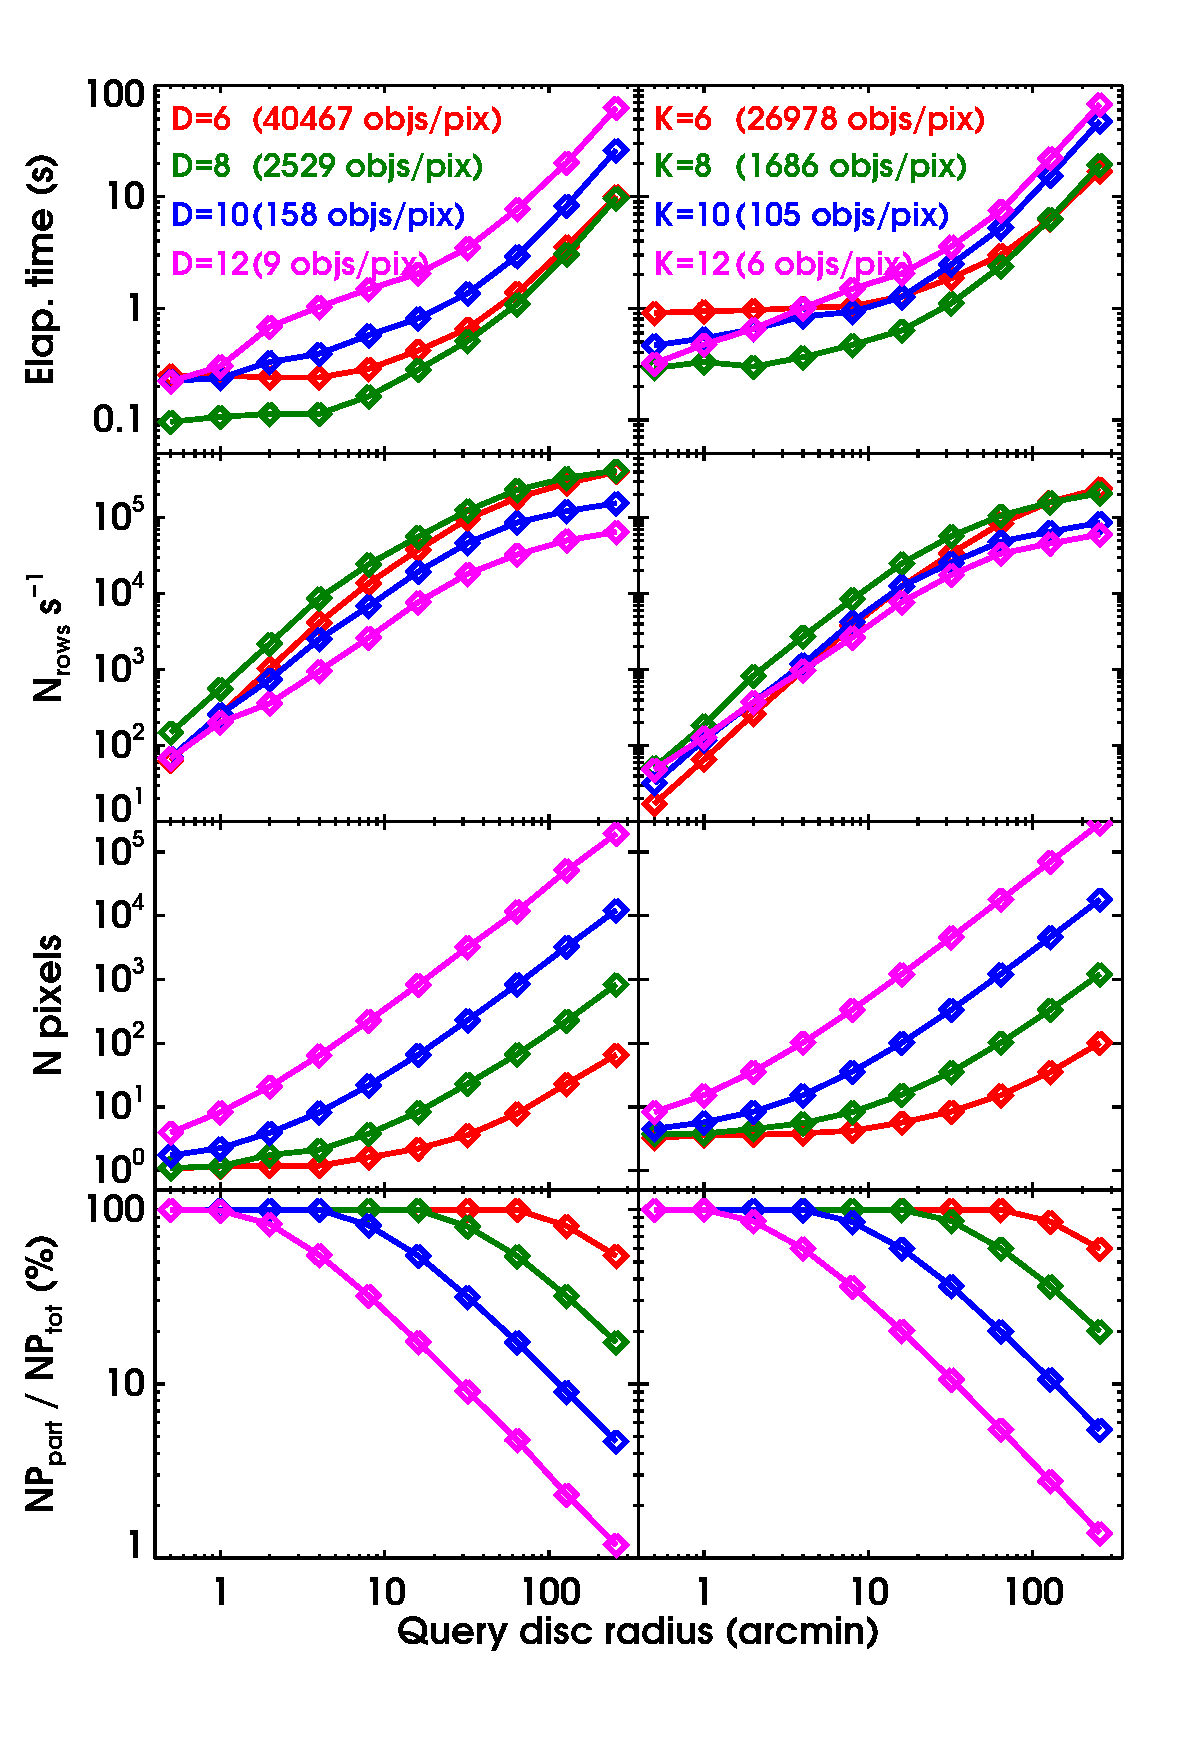
\includegraphics[height=8.5cm,clip=]{includes/fktimes_2}
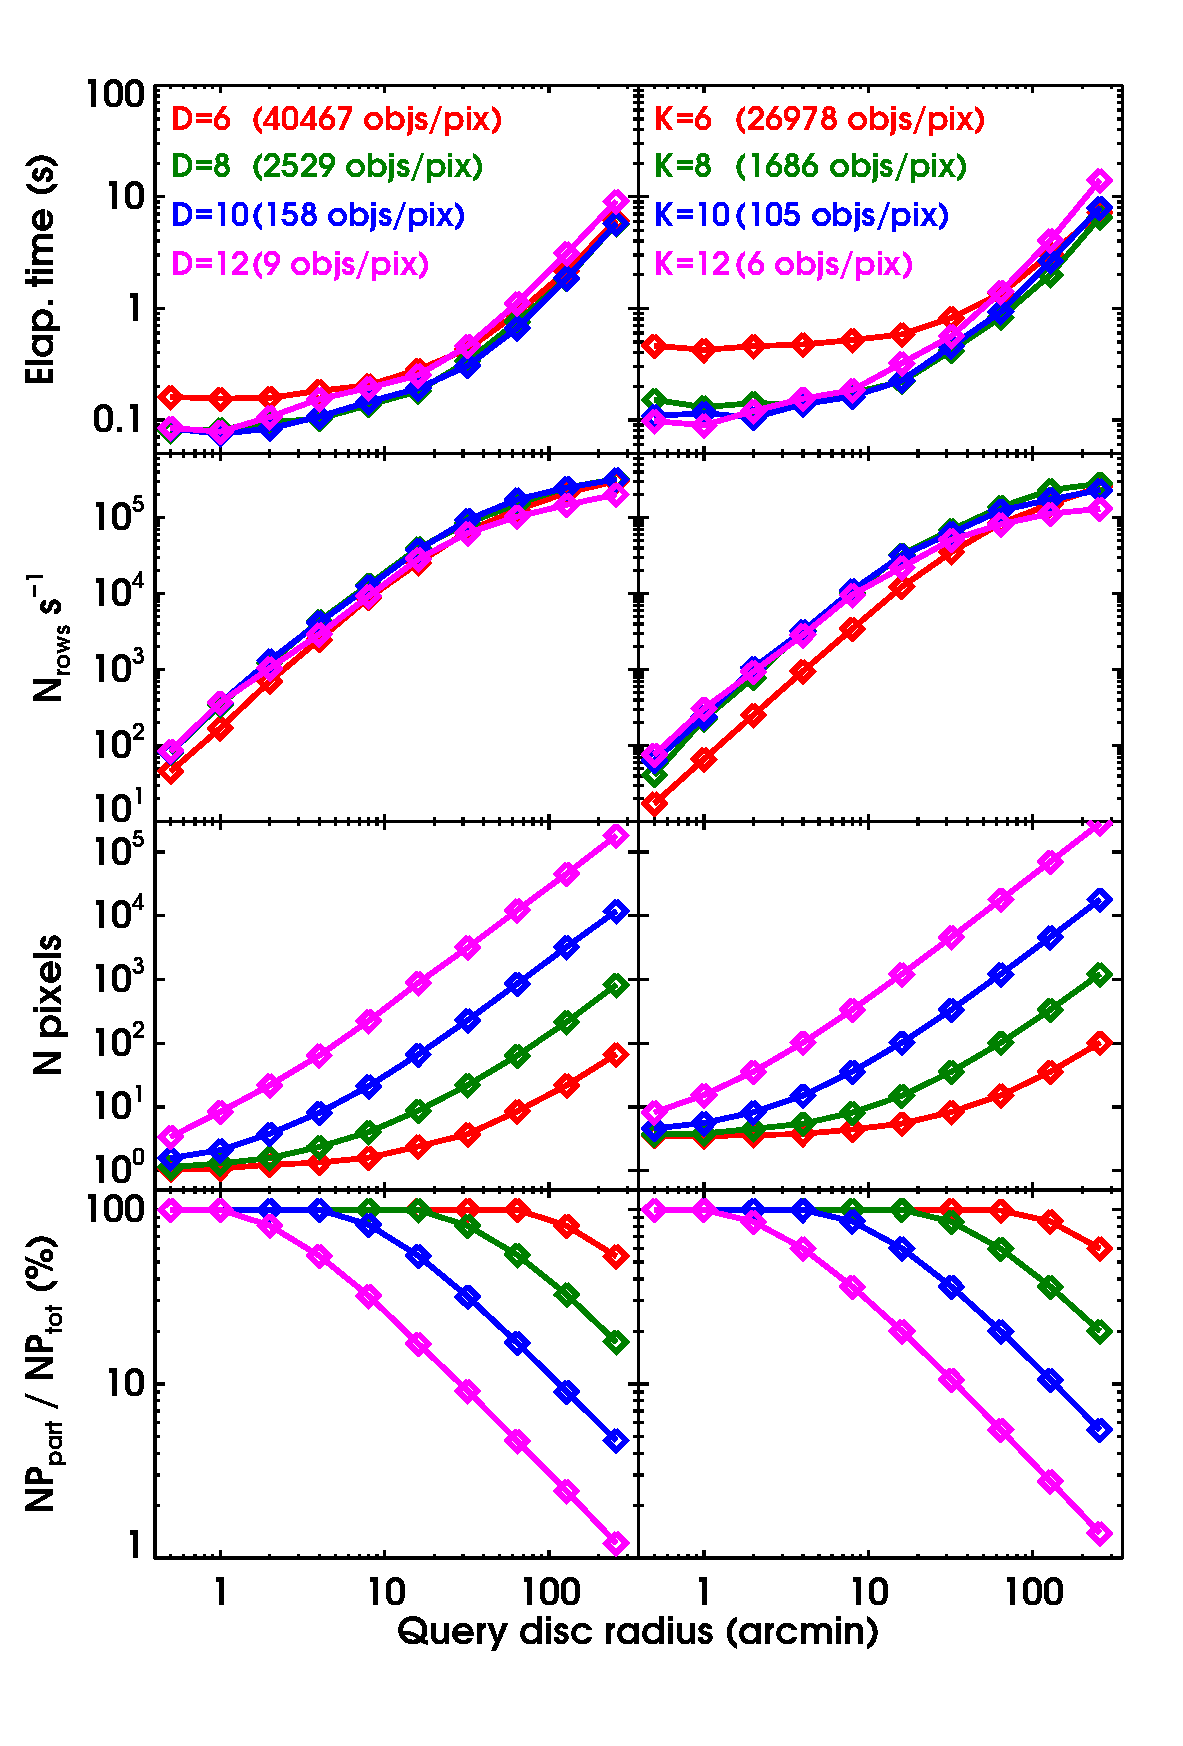
\includegraphics[height=8.5cm,clip=]{includes/fktimes1m_2}
\caption{Select query execution times and other parameters for a \dif\
 managed table with $\sim 3$ (\textit{left}) and $\sim 1$ (\textit{right})
 billion entries as a function of the disc radius.
 Results for four different pixel scales are reported both for
 HTM (\textit{left} in each panel) and HEALPix (\textit{right}).
 Each point represents
 the average of the results from 50 queries performed on random sky
 positions.
 }
\label{fig:bench}
\end{figure}
%
%\begin{figure}
%\centering
%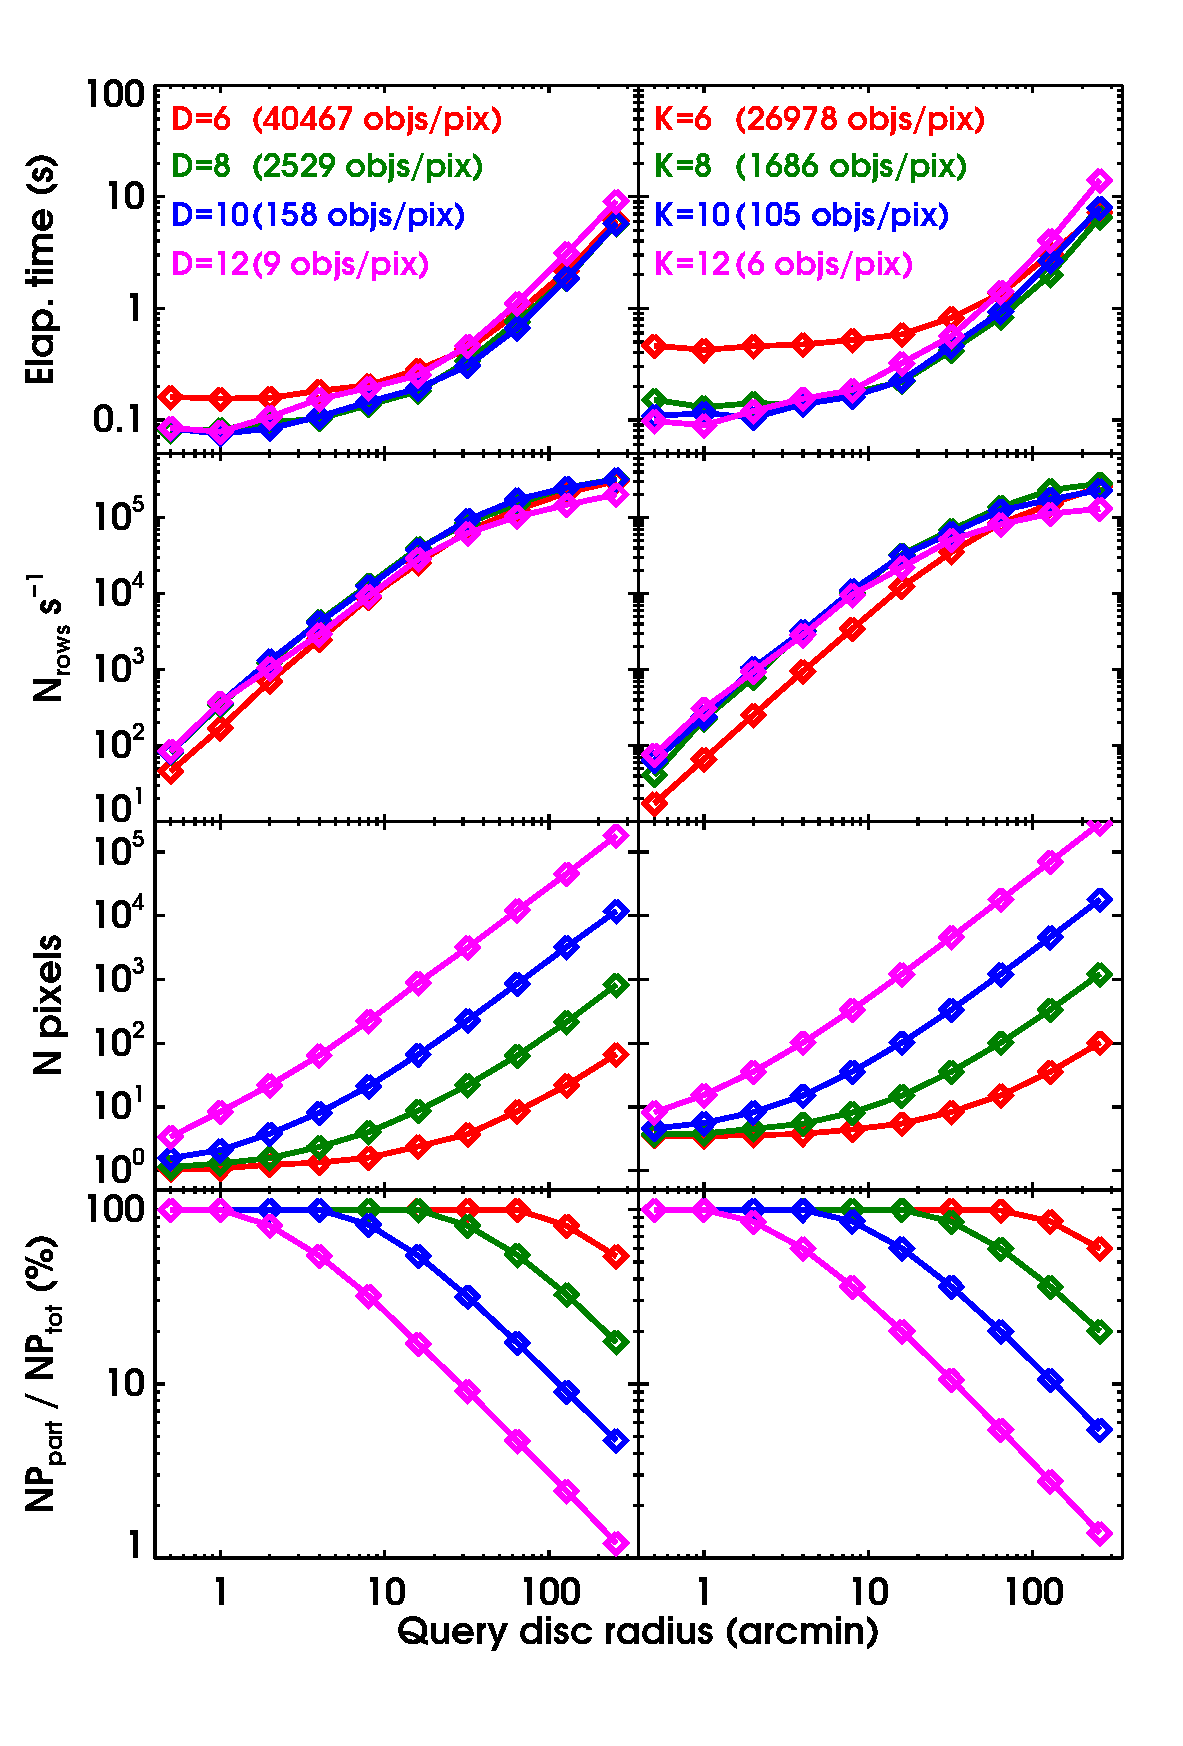
\includegraphics[height=8cm,clip=]{includes/fktimes1m_2}
%\caption{As for Fig. \ref{fig:bench3GP}  but for a table
% with $\sim 1$ billion entries.
% }
%\label{fig:bench1GP}
%\end{figure}
%

\smallskip
If you are intersted in \dif\ then you are likely dealing with a large
amount of data. As for any type of large dataset, apart using indices,
the queries on sky
regions greatly benefit from an ``ordered'' table on disk, i.e. with
data more localized phisically. This because the
disk data seek is minimized and the access is performed sequentially.
The only difference here is that on sky (or other multi-dimensional space)
a unique (or best) data sort scheme/order does not exist.
What is certain is that once
a sky pixelization, and then indexing scheme is choosen, it is adviceable
to sort the data to match the index. This way data of entries close on-sky
will also be close on-disk. In case multiple depths are used,
i.e. several indices match several spatial scales, the user should sort on
the index closer to the most likely queried region size.
As already mentioned in \S\ \ref{sec:pixschema}, using a pixel size of
$\sim 20^\prime$ (i.e. split the sky in $\sim 1/2$ million pixels) is a
choice which is adequate for a generic-use table with up to
some billion entries.

In case a table is only used for \verb|SELECT| queries, i.e. it is not
being modified, ordering the data on disk can be easily achieved using the
shell command (as root) \verb|myisamchk -R| \textit{index} {\tt Table}
(see \verb|myisamchk| manual). This assumes a \verb|MyISAM| table.
Note that sorting time depends both on the size of the table and the
``disorder'' of the data. Adding new data with random sky positions would
require a new sort to keep the table optimized. However if the added data
are a small fraction of the total, the operation would only take slitly longer
than a simple table copy operation.
Moreover, if the data within a pixel are sorted either in RA (longitude) or
Dec (latitude) then a \verb|SELECT| query which, in addition to a \dif\
function, in the \verb|WHERE| clause makes use of the sorted coordinate field
to delimit a range, then the query execution time can reduce by up an
order of magnitude! Actual speed depends on the size of the queried region
with respect to the pixel size. Without going into the details of pixelization
used and machine configurations but just to give an example from our
experience, selecting the objects falling into a $10^\prime\times10^\prime$
region from a one billion object catalogue reduces from $\sim 100-200$ ms,
using \verb|DIF_Rect| alone, to $\sim 20$ ms adding the RA boundary condition.

Sometimes it would also be a good idea to compress read-only tables
as this would reduce the seek and access time. In this case can use
\verb|myisampack|.
If you still need to improve performance, it is also adviceable to put the
table(s) on a RAID system, in particular level 10 or 50 would be safe and fast
both in read and write mode. Otherwise, the more the disks in the RAID
the faster a \verb|SELECT| query runs. Finally, when deciding which
filesystem one should prefer, it is better considering safety first.
All the commonly used filesystems have \textit{mount} options which can
significantly improve their performance at the expense of safety.
If one has very large tables, it is likely that the most common use is
the selection (i.e. read) of a subset of its entries. In this case
check on the web for a filesystem benchmark and, if the test is
present, select the one that performs best for ``extracting a subset of
data from a large file''.

When a table is intended for a very specialized use, routines or triggers
can be created to keep the table in ``good shape''.
We will not discuss this here but just mention the case when a table
is feeded on a more or less regular base with new entries. In this case
the usage of the \verb|PARTITION BY| option on the table together with
a trigger managed re-ordering or a periodic sorting via a scheduled
\verb|Event| would be a good solution. In other cases, the use of the
\verb|MERGE| DB engine would be adeguate and actullay more flexible than
the \verb|PARTITION BY| option. It is the DB manager that, depending on data
being managed, and eventually tests, should decide which is the best strategy.
In all cases the aim is always the same: reduce the amount of data the
DB server has to deal with taking into consideration that for a \verb|SELECT|
(or \verb|UPDATE|) query the more these data are fragmented on disk(s),
the more the time necessary to grab and deliver it to the user. 

Last but not least, do consider to take advantage of the MySQL query cache
(can use ``\texttt{SHOW VARIABLES LIKE "\%query\_cache\%"}'' to see settings for
your system).
In fact if you need a super-fast selection of the entries falling in a
given region and the coordinates of this region can be
\emph{predicted} before a routine/application actually will use it,
then a preliminary dummy \verb|SELECT| query can be executed.
When the actual query will be executed, MySQL will deliver the data without
the need to perform the search again, assuming they fit into the
available cache. Of course concurrent use of the cache memory does not
guarantees this will work in all cases because other queries performed between
the dummy and actual query could replace the data in the cache.

%---------------------------------------------------------------------
\newpage
\section{DIF function reference}
\label{sec:DIF_function_reference}

There are three kind of functions installed by \dif:
\begin{itemize}
\item wrapper to corresponding function in the HTM/HEALPix libraries;
\item functions related to the DB engine, that is to manipulate the
  content of the {\tt DIF.dif} table;
\item utility functions.
\end{itemize}
The reference documentation for each function is reported below.
%
%

\subsection{Wrapper to function in the HTM library}
These functions allow calling underlying functions in the HTM library
directly from SQL.
%

\subsubsection{{\tt HTMidByName}}
\syntax{HTMidByName(IdName STRING)}

\begin{parameters}
  \param{IdName}{STRING}: ID name of the trixel of interest;
\end{parameters}

\return{INT} HTM trixel Id.

\example
%
\begin{verbatim}
  select HTMidByName('S0000000');
    32768
\end{verbatim}
%
%

\subsubsection{{\tt HTMnameById}}
\syntax{HTMnameById(Id INT)}

\begin{parameters}
  \param{Id}{INT}: ID of the trixel of interest;
\end{parameters}

\return{STRING} HTM trixel Id name.

\example
%
\begin{verbatim}
  select HTMnameById(32768);
    S0000000
\end{verbatim}
%
%

\subsubsection{{\tt HTMBary}}
Return the HTM trixel barycenter coordinates given depth and trixel ID.

\syntax{HTMBary(Depth INT, Id INT)}

\begin{parameters}
  \param{Depth}{INT}: depth ($[0:25]$) of the pixelization scheme;
  \param{Id}{INT}: ID of the trixel of interest;
\end{parameters}

\return{STRING} Comma separated coordinates of the HTM trixel barycenter, in
  degrees.

\example
%
\begin{verbatim}
  select HTMBary(6,32768);
    0.4687499999999769, -0.46875
\end{verbatim}
%
%

\subsubsection{{\tt HTMBaryC}}
Return the HTM trixel barycenter coordinates given depth and
a pair of spherical coordinates.

\syntax{HTMBaryC(Depth INT, Ra DOUBLE, Dec DOUBLE)}

\begin{parameters}
  \param{Depth}{INT}: depth ($[0:25]$) of the pixelization scheme;
  \param{Ra}{DOUBLE}: right ascension (or longitude), in degrees;
  \param{Dec}{DOUBLE}: declination (or latitude), in degrees;
\end{parameters}

\return{STRING} Comma separated coordinates of the HTM trixel barycenter, in
  degrees.

\example
%
\begin{verbatim}
  select HTMBaryC(6,20,30);
    20.03084356871285, 30.26104286747405
\end{verbatim}
%
%

\subsubsection{{\tt HTMBaryDist}}
Return the distance from the HTM trixel barycenter given depth and a pair
of spherical coordinates.

\syntax{HTMBaryDist(Depth INT, Id INT, Ra DOUBLE, Dec DOUBLE)}

\begin{parameters}
  \param{Depth}{INT}: depth ($[0:25]$) of the pixelization scheme;
  \param{Id}{INT}: ID of the trixel of interest;
  \param{Ra}{DOUBLE}: right ascension (or longitude), in degrees;
  \param{Dec}{DOUBLE}: declination (or latitude), in degrees;
\end{parameters}

\return{DOUBLE} Angular distance from the trixel barycenter, in arcmin.

\example
%
\begin{verbatim}
  select HTMBaryDist(6,htmID_6,RAcs/3.6e5,DECcs/3.6e5) from
         UCAC_2orig_htm_6 where DIF_Circle(100,0,10);
    ...
    260 rows in set
\end{verbatim}




\subsubsection{{\tt HTMLookup}}
Return the ID of the HTM trixel given depth and a pair of spherical coordinates.

\syntax{HTMLookup(Depth INT, Ra DOUBLE, Dec DOUBLE)}

\begin{parameters}
  \param{Depth}{INT}: depth ($[0:25]$) of the pixelization scheme;
  \param{Ra}{DOUBLE}: right ascension (or longitude), in degrees;
  \param{Dec}{DOUBLE}: declination (or latitude), in degrees;
\end{parameters}

\return{BIGINT} ID of the HTM trixel.

\example
%
\begin{verbatim}
  select HTMLookup(6,20,30);
    64152
\end{verbatim}




\subsubsection{{\tt HTMNeighb}}
Return the IDs of the HTM trixels touching the given pixel ID (neighbors).

\syntax{HTMNeighb(Depth INT, Id INT)}

\begin{parameters}
  \param{Depth}{INT}: depth level ($[0:25]$) of the pixelization;
  \param{Id}{INT}: ID of the trixel of interest;
\end{parameters}

\return{STRING} A comma separated string with the (typically) 12 HTM trixels
IDs sorted in ascending order. For trixels touching any multiple of $90\deg$
angles the neighbors are (typically) 10.

\example
%
\begin{verbatim}
  select HTMNeighb(6, 32768);
    32769, 32770, 32771, 47104, 47106, 47107, 49152, 63488, 63489, 63491
\end{verbatim}
%
%

\subsubsection{{\tt HTMsNeighb}}
Return the IDs of the HTM trixels, at the same or higher depth, touching the
given pixel ID ("smaller" neighbors).

\syntax{HTMsNeighb(Depth INT, Id INT, oDepth INT)}

\begin{parameters}
  \param{Depth}{INT}: depth level ($[0:25]$) of the pixelization;
  \param{Id}{INT}: ID of the trixel of interest;
  \param{oDepth}{INT}: depth level of the map for the border trixels ($\ge$ \emph{Depth});
\end{parameters}

\return{STRING} A comma separated string with the HTM trixel IDs at level \emph{oDepth}.

\example
%
\begin{verbatim}
  select HTMsNeighb(6,32768,8);
    524312, 524324, 524340, 524341, 524343, 524344, 524346, 524347, 524348,
    753664, 753666, 753667, 753672, 753673, 753675,753677, 753700, 753716,
    786432, 1015808, 1015809, 1015811, 1015812, 1015814, 1015815, 1015822,
    1015832, 1015864
\end{verbatim}
%
%

\subsubsection{{\tt HTMNeighbC}}
Return the IDs of the HTM trixels and its neighbours given a pair of
spherical coordinates.

\syntax{HTMNeighbC(Depth INT, Ra DOUBLE, Dec DOUBLE)}

\begin{parameters}
  \param{Depth}{INT}: depth level ($[0:25]$) of the pixelization;
  \param{Ra}{DOUBLE}: right ascension (or longitude), in degrees;
  \param{Dec}{DOUBLE}: declination (or latitude), in degrees;
\end{parameters}

\return{STRING} A comma separated string with the (typically) 13 HTM trixel
IDs. For angles multiple of $90\deg$ the number of neighbors is (typically) 11.
Order is: the central one, the remaining 12 sorted in ascending order.

\example
%
\begin{verbatim}
  select HTMNeighbC(6, 100,60);
    58772, 58773, 58774, 58775, 58792, 58800, 58802, 58803, 58820, 58840,
    58841, 58843, 58872
\end{verbatim}
%
%

\subsection{Wrapper to function in the HEALPix library}
These functions allows calling underlying functions in the HEALPix library
directly from SQL.
%
%

\subsubsection{{\tt HEALPBary}}
Return the HEALPix barycenter (center) coordinates given scheme, order and
pixel ID.

\syntax{HEALPBary(Nested INT, Order INT, Id INT)}

\begin{parameters}
  \param{Nested}{INT}: map ordering, 0 for RING, 1 for NESTED;
  \param{Order}{INT}: order ($[0:29]$) of the pixelization scheme;
  \param{Id}{INT}: ID of the pixel of interest;
\end{parameters}

\return{STRING} Comma separated coordinates of the HEALPix pixel center, in
  degrees.

\example
%
\begin{verbatim}
  select HEALPBary(1,8,500);
    48.1640625, 6.429418462523309
\end{verbatim}
%
%

\subsubsection{{\tt HEALPBaryC}}
Return the HEALPix barycenter (center) coordinates given scheme, order and
a pair of spherical coordinates.

\syntax{HEALPBaryC(Nested INT, Order INT, Ra DOUBLE, Dec DOUBLE)}

\begin{parameters}
  \param{Nested}{INT}: map ordering, 0 for RING, 1 for NESTED;
  \param{Order}{INT}: order ($[0:29]$) of the pixelization scheme;
  \param{Ra}{DOUBLE}: right ascension (or longitude), in degrees;
  \param{Dec}{DOUBLE}: declination (or latitude), in degrees;
\end{parameters}

\return{STRING} Comma separated coordinates of the HEALPix pixel center, in
  degrees.

\example
%
\begin{verbatim}
  select HEALPBaryC(0,8,20.5,30.8);
    20.390625, 30.86525625461861
\end{verbatim}
%
%

\subsubsection{{\tt HEALPBaryDist}}
Return the distance from the HEALPix barycenter (center) given scheme,
order and a pair of spherical coordinates.

\syntax{HEALPBaryDist(Nested INT, Order INT, Id INT, Ra DOUBLE, Dec DOUBLE)}

\begin{parameters}
  \param{Nested}{INT}: map ordering, 0 for RING, 1 for NESTED;
  \param{Order}{INT}: order ($[0:29]$) of the pixelization scheme;
  \param{Id}{INT}: ID of the pixel of interest;
  \param{Ra}{DOUBLE}: right ascension (or longitude), in degrees;
  \param{Dec}{DOUBLE}: declination (or latitude), in degrees;
\end{parameters}

\return{DOUBLE} Angular distance from the pixel center, in arcmin.

\example
%
\begin{verbatim}
  select HEALPBaryDist(1,8,healpID_nest_8,RAcs/3.6e5,DECcs/3.6e5) from
         UCAC_2orig_healp_nest_8 where DIF_Circle(100,0,10);
    ...
    260 rows in set
\end{verbatim}
%
%

\subsubsection{{\tt HEALPLookup}}
Return the ID of the HEALPix pixel given scheme, order and a pair of
spherical coordinates.

\syntax{HEALPLookup(Nested INT, Order INT, Ra DOUBLE, Dec DOUBLE)}

\begin{parameters}
  \param{Nested}{INT}: map ordering, 0 for RING, 1 for NESTED;
  \param{Order}{INT}: order ($[0:29]$) of the pixelization scheme;
  \param{Ra}{DOUBLE}: right ascension (or longitude), in degrees;
  \param{Dec}{DOUBLE}: declination (or latitude), in degrees;
\end{parameters}

\return{BIGINT} ID of the HEALPix pixel.

\example
%
\begin{verbatim}
  select HEALPLookup(0,8,20,30);
    196152
\end{verbatim}
%
%

\subsubsection{{\tt HEALPNeighb}}
Return the IDs of the HEALPix pixels touching the given pixel ID (neighbors).

\syntax{HEALPNeighb(Nested INT, Order INT, Id INT)}

\begin{parameters}
  \param{Nested}{INT}: map ordering, 0 for RING, 1 for NESTED;
  \param{Order}{INT}: order ($[0:29]$) of the pixelization scheme;
  \param{Id}{INT}: ID of the pixel of interest;
\end{parameters}

\return{STRING} A comma separated string with the (typically) 8 HEALPix pixels
IDs. At some peculiar angles the W, N, E or S neighbors could not exist.
Order is: the SW, W, NW, N, NE, E, SE and S neighbor.

\example
%
\begin{verbatim}
  select HEALPNeighb(0, 8, 1000);
    1091, 999, 912, 829, 913, 1001, 1092, 1187
\end{verbatim}
%
%

\subsubsection{{\tt HEALPNeighbC}}
Return the IDs of the HEALPix pixel and its neighbours given a pair of
spherical coordinates.

\syntax{HEALPNeighbC(Nested INT, Order INT, Ra DOUBLE, Dec DOUBLE)}

\begin{parameters}
  \param{Nested}{INT}: map ordering, 0 for RING, 1 for NESTED;
  \param{Order}{INT}: order ($[0:29]$) of the pixelization scheme;
  \param{Ra}{DOUBLE}: right ascension (or longitude), in degrees;
  \param{Dec}{DOUBLE}: declination (or latitude), in degrees;
\end{parameters}

\return{STRING} A comma separated string with the (typically) 9 HEALPix pixels
IDs. At some peculiar angles the W, N, E or S neighbors could not exist.
Order is: central one, the SW, W, NW, N, NE, E, SE and S neighbor.

\example
%
\begin{verbatim}
  select HEALPNeighbC(1, 8, 100,60);
    113911, 113910, 113916, 113917, 114088, 114082, 114080, 113909, 113908
\end{verbatim}
%
%

\subsubsection{{\tt HEALPBound}}
Return the spherical coordinates of the HEALPix pixel boundaries given scheme,
order and ID. The (optional) input oversampling step determines the
number of returned coordinates along the boundaries. If Step = 1 then the 4
pixel corners (N, W, S and E) are returned.

\syntax{HEALPBound(Nested INT, Order INT, Id INT [, Step INT])}

\begin{parameters}
  \param{Nested}{INT}: map ordering, 0 for RING, 1 for NESTED;
  \param{Order}{INT}: order ($[0:29]$) of the pixelization scheme;
  \param{Id}{INT}: ID of the pixel of interest;
  \param{Step}{INT}: oversampling factor along each boundary;
\end{parameters}

\return{STRING} A comma separated string with the HEALPix pixel boundaries
coordinates.

\example
%
\begin{verbatim}
  select HEALPBound(1, 8, 1000);
    43.9453125, 8.38553864708132, 43.76953125, 8.234747571463606,
    43.9453125, 8.084013907099306, 44.12109375, 8.234747571463606
\end{verbatim}
%
%

\subsubsection{{\tt HEALPBoundC}}
Return the spherical coordinates of the HEALPix pixel boundaries given a pair
of spherical coordinates. The (optional) input oversampling step determines the
number of returned coordinates along the boundaries. If Step = 1 then the 4
pixel corners (N, W, S and E) are returned.

\syntax{HEALPBoundC(Nested INT, Order INT, Ra DOUBLE, Dec DOUBLE [, Step INT])}

\begin{parameters}
  \param{Nested}{INT}: map ordering, 0 for RING, 1 for NESTED;
  \param{Order}{INT}: order ($[0:29]$) of the pixelization scheme;
  \param{Ra}{DOUBLE}: right ascension (or longitude), in degrees;
  \param{Dec}{DOUBLE}: declination (or latitude), in degrees;
  \param{Step}{INT}: oversampling factor along each boundary;
\end{parameters}

\return{STRING} A comma separated string with the HEALPix pixel boundaries
coordinates.

\example
%
\begin{verbatim}
  select HEALPBoundC(1, 8, 100,60);
    100, 60.05627904951215, 99.93865030674847, 59.86707420480209,
    100.4268292682927, 59.67778522657881, 100.4907975460123, 59.86707420480209
\end{verbatim}
%
%

\subsubsection{{\tt HEALPMaxS}}
Return the HEALPix pixel max size (in arcmin) from center to corner
(both RING or NESTED), given the order.

\syntax{HEALPMaxS(Order INT)}

\begin{parameters}
  \param{Order}{INT}: order ($[0:29]$) of the pixelization scheme;
\end{parameters}

\return{DOUBLE} Angular distance in arcmin from the center of the pixel to the
furthest corner.

\example
%
\begin{verbatim}
  select HealPMaxS(6);
    57.24888364432666
  select HealPMaxS(8);
    14.34420720055738
  select HealPMaxS(12);
    0.8971372281806288
\end{verbatim}
%
%

\subsubsection{{\tt Sphedist}}
Compute the angular distance given the coordinates of two points
on a sphere.

\syntax{Sphedist(Ra1 DOUBLE, Dec1 DOUBLE, Ra2 DOUBLE, Dec2 DOUBLE)}

\begin{parameters}
  \param{Ra1}{DOUBLE}: right ascension (or longitude) of the
  first point, in degrees;
  \param{Dec1}{DOUBLE}: declination (or latitude) of the first
  point, in degrees;
  \param{Ra2}{DOUBLE}: right ascension (or longitude) of the
  second point, in degrees;
  \param{Dec2}{DOUBLE}: declination (or latitude) of the second
  point, in degrees;
\end{parameters}

\return{DOUBLE} Angular distance between the points, in arcmin.



%
\subsection{DB engine-related functions: region selections}
These functions are dedicated to the definition of a search
region. Typically they are used in the {\tt WHERE} clause of a {\tt
  SELECT} query.


\subsubsection{{\tt DIF\_Circle}}
Define a circular search region entered at the given coordinates and with the
given radius. 
%searchGenerate all IDs of the HTM/HEALPix trixels which lie, partially or
%entirely, inside a circle centered at the given coordinates and with
%the given radius. The generated IDs can be read from the
%\verb|DIF.dif| table. This function should only be used in a
%\verb|WHERE| clause which reads from a \verb|*_htm[_N]| view or as the
%only argument of a \verb|SELECT| query.

\syntax{DIF\_Circle(Ra DOUBLE, Dec DOUBLE, Rad DOUBLE)}

\begin{parameters}
  \param{Ra}{DOUBLE}: right ascension (or longitude) of the
  center, in degrees;
  \param{Dec}{DOUBLE}: declination (or latitude) of the center,
  in degrees;
  \param{Rad}{DOUBLE}: radius of the cicle, in arcmin;
\end{parameters}

\return{BIGINT} Always 1;

\example
%
\begin{verbatim}
  SELECT * FROM Messier_htm_6 WHERE DIF_Circle(82, 22, 100);
\end{verbatim}




\subsubsection{{\tt DIF\_Rect}}
Define a rectangular search region whose sides lie along lines of
constant right ascension (longitude) and declination (latitude).

\syntax{DIF\_Rect(Ra DOUBLE, Dec DOUBLE, side DOUBLE [, side2 DOUBLE])}

\begin{parameters}
  \param{Ra}{DOUBLE}: right ascension (or longitude) of the
  center, in degrees;
  \param{Dec}{DOUBLE}: declination (or latitude) of the center,
  in degrees;
  \param{side}{DOUBLE}: the length of the sides along the right ascension,
  in arcmin;
  if the fourth argument is omitted this is the length of all sides of
  the rectangle, i.e. it is a square;
  \param{side2}{DOUBLE} (optional): length of the sides along
  the declination, in arcmin;
\end{parameters}

\return{BIGINT} Always 1.

\example
%
\begin{verbatim}
  select htmID_8,RAcs/3.6e5,DECcs/3.6e5 from
         UCAC_2orig_htm_6 where DIF_Rect(100,30,10);
    ...
    74 rows in set
\end{verbatim}
%
%

\subsubsection{{\tt DIF\_Rectv}}
Define a rectangle (or four sides polygon) search region with given
coordinates of the vertices. This function can be called either with four or eight
arguments. In the first case the arguments are assumed to be the
coordinates of two opposite vertices of the rectangular region and thus
the sides of the region lie along lines of constant right ascension
and declination. In the second case the arguments are
the coordinates of the vertices of a four sides polygon.
In this case the largest rectangle included in the polygon is used. 
In the future any type of polygons will be supported.

\syntax{DIF\_RectV(Ra1 DOUBLE, Dec1 DOUBLE, Ra2
  DOUBLE, Dec2 DOUBLE [, Ra3 DOUBLE, Dec3 DOUBLE,
  Ra4 DOUBLE, Dec4 DOUBLE])}

\begin{parameters}
  \param{Ra1}{DOUBLE}: right ascension (or longitude) of the
  first vertex, in degrees;
  \param{Dec1}{DOUBLE}: declination (or latitude) of the first
  vertex, in degrees;
  \param{Ra2}{DOUBLE}: right ascension (or longitude) of the
  second vertex, in degrees;
  \param{Dec2}{DOUBLE}: declination (or latitude) of the second
  vertex, in degrees;
  \param{Ra3}{DOUBLE} (optional): right ascension (or longitude)
  of the third vertex, in degrees;
  \param{Dec3}{DOUBLE} (optional): declination (or latitude) of
  the third vertex, in degrees;
  \param{Ra4}{DOUBLE} (optional): right ascension (or longitude)
  of the fourth vertex, in degrees;
  \param{Dec4}{DOUBLE} (optional): declination (or latitude) of
  the fourth vertex, in degrees;
\end{parameters}

\return{BIGINT} Always 1.

\example
%
\begin{verbatim}
  select htmID_6,RAcs/3.6e5,DECcs/3.6e5 from
         UCAC_2orig_htm_6 where DIF_Rectv(10,30,10.3,30.3);
    ...
    776 rows in set
\end{verbatim}
%
%

\subsubsection{{\tt DIF\_NeighbC}}
Define a search region composed of a HTM/HEALPix pixel and its
neighbors given a pair of spherical coordinates.

\syntax{DIF\_NeighbC(Ra DOUBLE, Dec DOUBLE)}

\begin{parameters}
  \param{Ra}{DOUBLE}: right ascension (or longitude), in degrees;
  \param{Dec}{DOUBLE}: declination (or latitude), in degrees;
\end{parameters}
%
\return{BIGINT} How many HTM/HEALPix pixels have been selected.
%

\example
%
\begin{verbatim}
  SELECT * FROM Messier_htm_6 WHERE DIF_NeighbC(82, 22);
\end{verbatim}
%
%
Note that for tables with multiple depths you can only use the smaller
one (larger trixel).

%
\subsubsection{{\tt DIF\_sNeighb}}
Given a HTM trixel at a given depth, it defines a search region composed of
the neighbors trixels at a higher depth (smaller). \\
NOTE: the table must be \dif\ indexed at both depths!

\syntax{DIF\_sNeighb(Depth INT, Id INT, oDepth INT)}

\begin{parameters}
  \param{Depth}{INT}: depth level ($[0:25]$) of the pixelization;
  \param{Id}{INT}: ID of the trixel of interest;
  \param{oDepth}{INT}: depth level of the map for the border trixels ($\ge$ \emph{Depth});
\end{parameters}

\example
%
\begin{verbatim}
  SELECT * FROM Messier_htm_6 WHERE DIF_sNeighb(6, 62392, 8);

  | 1 | BN   | Tau   |  8.2 | 83.625 | 22.0167  ...
\end{verbatim}

Note that you need first to index on depth 8 the Messier catalogue:
%
\begin{verbatim}
  dif --index-htm DIF Messier 8 Ra Decl
\end{verbatim}
%
Also being the catalogue quite small, the values above where calculated on
purpose with a lookup to the trixels IDs around the coordinates of the
example above:
\begin{verbatim}
  select htmlookup(6,83.625,22.0167);
  62340
  select htmlookup(6,83.45,22.0167);
  62392
\end{verbatim}

%
%
\subsection{DB engine-related functions: auxiliary functions}
These are DB engine-related auxiliary functions. The three functions
{\tt DIF\_setHTMDepth}, {\tt DIF\_setHEALPOrder} and {\tt
  DIF\_FineSearch} are not meant to be used by users, but only inside
\dif\ views, thus their reference will not be given here.


\subsubsection{{\tt DIF\_clear}}
Clear all user defined region and associated HTM/HEALPix pixel
list. Although not mandatory, this function should be called each time
a user wish to use \dif\ facilities since MySQL does not always destroy
the thread of a previous user connection. 

\syntax{DIF\_clear()}
%
%

\subsubsection{{\tt DIF\_cpuTime}}
This function returns the cumulative usage of CPU time by the DIF functions.
It is useful to quantify the impact of DIF usage with respect to the total
time required to execute a query.

\syntax{DIF\_cpuTime()}

\return{BIGINT} Cumulative CPU time (in seconds) since last reset.

\example
%
\begin{verbatim}
  select DIF_cpuTime()/1.;
    0.36
\end{verbatim}
%
%

\subsection{Utility functions}
This functions return information about \dif\ indexed tables. 
%

\subsubsection{{\tt getHTMDepth}}
Return the ``smallest'' (or only) depth of the HTM index created on a table.

\syntax{DIF.getHTMDepth(db CHAR(64), table CHAR(64))}

\begin{parameters}
  \param{db}{CHAR(64)}: name of the database which contains the table;
  \param{table}{CHAR(64)}: name of the table;
\end{parameters}

\return{INT} The ``smallest'' depth of HTM indexes in given table.

\example
%
\begin{verbatim}
  select DIF.getHTMDepth('MyCats','ascc25') as min_depth;
+-----------+
| min_depth |
+-----------+
|         4 |
+-----------+
\end{verbatim}
%
%


\subsubsection{{\tt getHEALPOrder}}
Return the ``smallest'' (or only) resolution parameter (order) of the HEALPix
index(es) created on a table.

\syntax{DIF.getHEALPOrder(db CHAR(64), table CHAR(64))}

\begin{parameters}
  \param{db}{CHAR(64)}: name of the database which contains the table;
  \param{table}{CHAR(64)}: name of the table;
\end{parameters}

\return{INT} Smallest resolution parameter of the HEALPix indexes in the
 given table.

\example
%
\begin{verbatim}
  select DIF.getHEALPOrder('MyCats','UCAC_2orig') as min_order;
+-----------+
| min_order |
+-----------+
|         8 |
+-----------+
\end{verbatim}
%
%


\subsubsection{{\tt getHEALPNested}}
Return the HEALPix map ID ordering scheme used to create the index on a table.

\syntax{DIF.getHEALPNested(db CHAR(64), table CHAR(64), order INTEGER)}

\begin{parameters}
  \param{db}{CHAR(64)}: name of the database which contains the table;
  \param{table}{CHAR(64)}: name of the table;
  \param{order}{INTEGER}: order of the pixelization;
\end{parameters}

\return{INT} Map ordering, 0 for RING, 1 for NESTED.

%
\begin{verbatim}
  select DIF.getHEALPNested('MyCats','UCAC_2orig',8) as is_nested;
+-----------+
| is_nested |
+-----------+
|         1 |
+-----------+
\end{verbatim}
%
%


\subsubsection{{\tt difview\_Check}}
Recursively shows the SQL expression to get rid of tables present in {\tt DIF.tbl} but no
corresponding view exists (check is done in {\tt INFORMATION\_SCHEMA.VIEWS}).
Note that the check ignores the possible presence of multiple views for a
table.

\syntax{call DIF.difview\_Check()}

\begin{parameters}
  \param{}{}: no parameters;
\end{parameters}

\return{VARCHAR, VARCHAR} The name of the table(s) with no view and the SQL
command to execute to remove the entry form {\tt DIF.tbl}.

\example
%
\begin{verbatim}
  call DIF.difview_Check();
+------------------------+---------------------------------------------------------+
| in_DIF_tbl_but_no_view | to_remove_run_command                                   |
+------------------------+---------------------------------------------------------+
| test.ascctest          | DELETE FROM DIF.tbl where db="test" AND name="ascctest" |
+------------------------+---------------------------------------------------------+
\end{verbatim}
%
%



\subsubsection{{\tt difview\_htmClean}}
Shows and optionally removes the HTM views present in {\tt INFORMATION\_SCHEMA.VIEWS}
(checking for {\tt \_htm} string) but no corresponsding entry is present in {\tt DIF.tbl}.

\syntax{call DIF.difview\_htmClean(IN doclean BOOLEAN)}

\begin{parameters}
  \param{doclean}{BOOLEAN}: if 1 then drops the views for tables not listed in {\tt DIF.tbl};
\end{parameters}

\return{VARCHAR} The message(s) about unlisted tables in {\tt DIF.tbl}.

\example
%
\begin{verbatim}
  call DIF.difview_htmClean(0);
+---------------------------------------------+
| Message                                     |
+---------------------------------------------+
| test.simplebsc_htm_14 not listed in DIF.tbl |
+---------------------------------------------+
\end{verbatim}
%
%


\subsubsection{{\tt difview\_healpClean}}
Shows and optionally removes the HEALPix views present in {\tt INFORMATION\_SCHEMA.VIEWS}
(checking for {\tt \_healp\_} string) but no corresponsding entry is present in {\tt DIF.tbl}.

\syntax{call DIF.difview\_healpClean(IN doclean BOOLEAN)}

\begin{parameters}
  \param{doclean}{BOOLEAN}: if 1 then drops the views for tables not listed in {\tt DIF.tbl};
\end{parameters}

\return{VARCHAR} The message(s) about unlisted tables in {\tt DIF.tbl}.

\example
%
\begin{verbatim}
  call DIF.difview_healpClean(0);
+---------------------------------------------------+
| Message                                           |
+---------------------------------------------------+
| test.simplebsc_healp_nest_8 not listed in DIF.tbl |
+---------------------------------------------------+
\end{verbatim}
%
%



\subsubsection{{\tt getRa}}
Simply read the \texttt{Ra\_field} from \texttt{DIF.tbl}, i.e. return the
SQL expression to get the right ascension / longitude as degrees for
entries of a given table.

\syntax{DIF.getRa(db CHAR(64), table CHAR(64))}

\begin{parameters}
  \param{db}{CHAR(64)}: name of the database which contains the table;
  \param{table}{CHAR(64)}: name of the table;
\end{parameters}

\return{VARCHAR} The SQL expression to get the right ascension (degrees).

\example
%
\begin{verbatim}
  select DIF.getRa('MyCats','ascc25');
+------------------------------+
| DIF.getra('MyCats','ascc25') |
+------------------------------+
| RAmas/3.6e6                  |
+------------------------------+
\end{verbatim}
%
%


\subsubsection{{\tt getDec}}
Simply read the \texttt{Dec\_field} from \texttt{DIF.tbl}, i.e. return the
SQL expression to get the declination / latitude as degrees for
entries of a given table.

\syntax{DIF.getDec(db CHAR(64), table CHAR(64))}

\begin{parameters}
  \param{db}{CHAR(64)}: name of the database which contains the table;
  \param{table}{CHAR(64)}: name of the table;
\end{parameters}

\return{VARCHAR} The SQL expression to get the declination (degrees).

\example
%
\begin{verbatim}
  select DIF.getDec('MyCats','ascc25');
+-------------------------------+
| DIF.getDec('MyCats','ascc25') |
+-------------------------------+
| DECmas/3.6e6                  |
+-------------------------------+
\end{verbatim}
%
%



\subsubsection{{\tt RAcol}}
Return the column name containing the RA in a given table.
It performs field comparison between column names in \texttt{INFORMATION\_SCHEMA.COLUMNS}
and \texttt{Ra\_field} in \texttt{DIF.tbl} 

\syntax{DIF.RAcol(db CHAR(64), table CHAR(64))}

\begin{parameters}
  \param{db}{CHAR(64)}: name of the database which contains the table;
  \param{table}{CHAR(64)}: name of the table;
\end{parameters}

\return{VARCHAR} The name of the column with right ascension.

\example
%
\begin{verbatim}
  select DIF.RAcol('MyCats','ascc25');
+------------------------------+
| DIF.RAcol('MyCats','ascc25') |
+------------------------------+
| RAmas                        |
+------------------------------+
\end{verbatim}
%
%

\subsubsection{{\tt DECcol}}
Return the column name containing the Dec in a given table.
It performs field comparison between column names in \texttt{INFORMATION\_SCHEMA.COLUMNS}
and \texttt{Dec\_field} in \texttt{DIF.tbl} 

\syntax{DIF.DECcol(db CHAR(64), table CHAR(64))}

\begin{parameters}
  \param{db}{CHAR(64)}: name of the database which contains the table;
  \param{table}{CHAR(64)}: name of the table;
\end{parameters}

\return{VARCHAR} The name of the column with declination.

\example
%
\begin{verbatim}
  select DIF.DECcol('MyCats','ascc25');
+------------------------------+
| DIF.DECcol('MyCats','ascc25') |
+------------------------------+
| DECmas                        |
+------------------------------+
\end{verbatim}
%
%



\subsubsection{{\tt difInfo}}
Show info about a given \dif\ function or procedure reading from \texttt{DIF.func}.

\syntax{call DIF.difInfo(IN udf VARCHAR(64))}

\begin{parameters}
  \param{udf}{VARCHAR}: the name of the function or procedure;
\end{parameters}

\return{6 VARCHAR} The fields present in {\tt DIF.func}, i.e.
\\
\texttt{name | params | ret | type | plugin\_lib | description}.

\example
%
\begin{verbatim}
  call DIF.difInfo('difInfo');
+---------+----------------------+------+-----------+------------+
| name    | params               | ret  | type      | plugin_lib |
+---------+----------------------+------+-----------+------------+
| difInfo | (IN udf VARCHAR(50)) | void | procedure | void       |
+---------+----------------------+------+-----------+------------+
          +-------------------------------------------+
          | description                               |
          +-------------------------------------------+
          | Show info for a DIF function or procedure |
          +-------------------------------------------+
\end{verbatim}
%
%


%The functions described in this section are installed by \dif. 
%Most \dif\ function are used to identify a region of the sky on which
%the query will be executed, whereas other are for getting information
%about the pixelitation used on a given table.
%Functions with the prefix \verb|DIF_| refer to the \dif\ database engine
%and they can only be used in the \verb|WHERE| clause referred
%to \verb|_htm| / \verb|_htm_N| or/and
%\verb|_healp| / \verb|_healp_N| table views. Region and neighbors selection
%functions can \textbf{also} be used as the only argument of a \verb|SELECT|
%query. This latter usage, introduced in version 0.4.0, will permanently apply
%(until a new \verb|DIF_| function is invoked) a spatial filter to any
%following query on the view(s).
%Functions with the prefix \verb|DIF.| are SQL function which act on the
%\verb|DIF.tbl| table. These and the other functions can be used anywhere in
%an SQL query string.



%\subsection{DIF\_HEALPCircle}
%Generate all IDs of HEALPix pixels which lies, partially or entirely,
%inside a spherical circle centered at the given coordinates and with
%given radius. The generated IDs can be read from the \verb|DIF.dif|
%table. This function should only be used in a \verb|WHERE| clause which reads
%from a \verb|*_healp[_N]| view
%or as the only argument of a \verb|SELECT| query.
%
%\syntax{DIF\_HEALPCircle(Ra DOUBLE, Dec DOUBLE, Rad DOUBLE)}
%
%\begin{parameters}
%  \param{Ra}{DOUBLE}: right ascension (or longitude) of the
%  center, in degrees;
%  \param{Dec}{DOUBLE}: declination (or latitude) of the center,
%  in degrees;
%  \param{Rad}{DOUBLE}: radius of the cicle, in arc minutes;
%\end{parameters}
%
%\return{BIGINT} How many HEALPix pixels have been selected.
%
%\noindent{\textbf{Example:}}
%%
%\begin{verbatim}
%select healpID_nest_8,RAcs/3.6e5,DECcs/3.6e5 from
%       UCAC_2orig_healp where DIF_HEALPCircle(100,30,10);
%  ...
%  186 rows in set
%\end{verbatim}
%%
%
%%
%\subsection{DIF\_HTMRect}
%Generate all IDs of the HTM trixels which lie, partially or entirely,
%inside a spherical rectangle centered at the given coordinates and
%with the given side(s) length. The sides lie along lines of constant right
%ascension (longitude) and declination (latitude).
%Objects falling out of the region are not returned (this is not the case for
%DIF\_HTMRectV),
%The generated IDs can be read from the
%\verb|DIF.dif| table. This function should only be used in a \verb|WHERE|
%clause which reads from a \verb|*_htm[_N]| view
%or as the only argument of a \verb|SELECT| query.
%
%%
%\syntax{DIF\_HTMRect(Ra DOUBLE, Dec DOUBLE, side DOUBLE [, side2 DOUBLE])}
%
%\begin{parameters}
%  \param{Ra}{DOUBLE}: right ascension (or longitude) of the
%  center, in degrees;
%  \param{Dec}{DOUBLE}: declination (or latitude) of the center,
%  in degrees;
%  \param{side}{DOUBLE}: the length of the sides along the right ascension,
%  in arcmin;
%  if the fourth argument is omitted this is the length of all sides of
%  the rectangle, i.e. it is a square;
%  \param{side2}{DOUBLE} (optional): length of the sides along
%  the declination, in arcmin;
%\end{parameters}
%
%\return{BIGINT} How many HTM trixels have been selected.
%
%\noindent{\textbf{Example:}}
%%
%\begin{verbatim}
%select htmID_8,RAcs/3.6e5,DECcs/3.6e5 from
%       UCAC_2orig_htm where DIF_HTMRect(100,30,10);
%  ...
%  74 rows in set
%\end{verbatim}
%%
%
%%
%%
%\subsection{DIF\_HTMRectV}
%Generate all IDs of the HTM trixels which lie, partially or entirely,
%inside a rectangle (or four sides polygon) with given coordinates
%of the vertices. All the objects falling into the pixels are returned.
%This function can be called either with four or eight
%arguments. In the first case the arguments are assumed to be the
%coordinates of two opposite vertices of the rectangular region and thus
%the sides of the region lie along lines of constant right ascension
%and declination. In the second case the arguments are
%the coordinates of the vertices of a four sides polygon.
%The generated IDs can be read from the
%\verb|DIF.dif| table. This function should only be used in a \verb|WHERE|
%clause which reads from a \verb|*_htm[_N]| view
%or as the only argument of a \verb|SELECT| query.
%
%\syntax{DIF\_HTMRectV(Ra1 DOUBLE, Dec1 DOUBLE, Ra2
%  DOUBLE, Dec2 DOUBLE [, Ra3 DOUBLE, Dec3 DOUBLE,
%  Ra4 DOUBLE, Dec4 DOUBLE])}
%
%\begin{parameters}
%  \param{Ra1}{DOUBLE}: right ascension (or longitude) of the
%  first vertex, in degrees;
%  \param{Dec1}{DOUBLE}: declination (or latitude) of the first
%  vertex, in degrees;
%  \param{Ra2}{DOUBLE}: right ascension (or longitude) of the
%  second vertex, in degrees;
%  \param{Dec2}{DOUBLE}: declination (or latitude) of the second
%  vertex, in degrees;
%  \param{Ra3}{DOUBLE} (optional): right ascension (or longitude)
%  of the third vertex, in degrees;
%  \param{Dec3}{DOUBLE} (optional): declination (or latitude) of
%  the third vertex, in degrees;
%  \param{Ra4}{DOUBLE} (optional): right ascension (or longitude)
%  of the fourth vertex, in degrees;
%  \param{Dec4}{DOUBLE} (optional): declination (or latitude) of
%  the fourth vertex, in degrees;
%\end{parameters}
%
%\return{BIGINT} How many HTM trixels have been selected.
%
%\noindent{\textbf{Example:}}
%%
%\begin{verbatim}
%select htmID_8,RAcs/3.6e5,DECcs/3.6e5 from
%       UCAC_2orig_htm where DIF_HTMRectV(10,30,10.3,30.3);
%  ...
%  776 rows in set
%\end{verbatim}
%%
%
%%
%%
%\subsection{DIF\_HTMNeighbC}
%Generate the IDs of the HTM trixel and its neighbors given a pair of
%spherical coordinates.
%The generated IDs can be read from the \verb|DIF.dif|
%table. This function should only be used in a \verb|WHERE| clause which reads
%from a \verb|*_htm[_N]| view
%or as the only argument of a \verb|SELECT| query.
%If no other clause is used, it will select all the objects falling in the
%central trixel and its neighbors.
%
%\syntax{DIF\_HTMNeighbC(Ra DOUBLE, Dec DOUBLE)}
%
%\begin{parameters}
%  \param{Ra}{DOUBLE}: right ascension (or longitude), in degrees;
%  \param{Dec}{DOUBLE}: declination (or latitude), in degrees;
%\end{parameters}
%
%\return{BIGINT} How many HTM trixels have been selected. Tipicallly 13
%(or 11 for angles multiple of 90 deg.).
%
%\noindent{\textbf{Example:}}
%%
%\begin{verbatim}
%select htmID_8,RAcs/3.6e5,DECcs/3.6e5 from
%       UCAC_2orig_htm where DIF_HTMNeighbC(30,10);
%  ...
%  4486 rows in set
%\end{verbatim}
%%
%
%%
%%
%\subsection{DIF\_HEALPNeighbC}
%Generate the IDs of the HEALPix pixel and its neighbors given
%a pair of spherical coordinates.
%The generated IDs can be read from the \verb|DIF.dif|
%table. This function should only be used in a \verb|WHERE| clause which reads
%from a \verb|*_healp[_N]| view
%or as the only argument of a \verb|SELECT| query.
%If no other clause is used, it will select all the objects falling in the
%central trixel and its neighbors.
%
%\syntax{DIF\_HEALPNeighbC(Ra DOUBLE, Dec DOUBLE)}
%
%\begin{parameters}
%  \param{Ra}{DOUBLE}: right ascension (or longitude), in degrees;
%  \param{Dec}{DOUBLE}: declination (or latitude), in degrees;
%\end{parameters}
%
%\return{BIGINT} How many HEALPix pixels have been selected. It is tipically 9
%(7 at peculiar angles).
%
%\noindent{\textbf{Example:}}
%%
%\begin{verbatim}
%select healpID_nest_8,RAcs/3.6e5,DECcs/3.6e5 from
%       UCAC_2orig_healp where DIF_HEALPNeighbC(30,10);
%  ...
%  145 rows in set
%\end{verbatim}
%%
%
%\subsection{DIF\_setHTMDepth}
%This function is not intended to be called by the user.
%
%\syntax{DIF\_setHTMDepth(depth INTEGER)}
%\begin{parameters}
%  \param{Depth}{INT}: depth level ($[0:25]$) of the pixelization;
%\end{parameters}
%
%\return{BIGINT} Always 1. It just sets the given input depth as available
% to the view(s).
%
%\subsection{DIF\_setHEALPOrder}
%This function is not intended to be called by the user.
%
%\syntax{DIF\_setHEALPOrder(nested INTEGER, order INTEGER)}
%\begin{parameters}
%  \param{Nested}{INT}: map ordering, 0 for RING, 1 for NESTED;
%  \param{Order}{INT}: order ($[0:29]$) of the pixelization scheme;
%\end{parameters}
%
%\return{BIGINT} Always 1. It just sets the given input order and scheme as
% available to the view(s).
%
%\subsection{DIF\_FineSearch}
%This function is not intended to be called by the user.
%It determines if entries falling in partially covered pixels are within
%the requested region or not. It must always be used in conjuction with a
%region selecting function.
%
%\syntax{DIF\_FineSearch([variable])}
%\begin{parameters}
%  \param{p}{DOUBLE}: the number of parameters depends on the function it is
%   used with.
%\end{parameters}
%
%\return{BIGINT} 1 if the entry is within the requested region, 0 otherwise.

%Note that the /1. is required to have the value printed as fractional number.

%
%---------------------------------------------------------------------
\newpage
\section{Generating fake sky tables}
\label{sec:fakesky}
In the \verb|src| sub-directory of the package there are three stand-alone
programs suitable to create table of fake sky
objects: \verb|fakesky_H6|, \verb|fakesky_HPx|, \verb|fakesky_RND|.
Here we describe what's their output and how to use them.
Some query examples are also presented with the ``expected'' results.

\bigskip
***More To Be Written***

\noindent Simple examples:
\begin{verbatim}
  ./fakesky_HPx -h
  ./fakesky_HPx
  ./fakesky_HPx -o 8
  ./fakesky_H6 -h
  ./fakesky_H6
  ./fakesky_H6 -D .5
\end{verbatim}
%
\emph{Please see source code}

%
%---------------------------------------------------------------------
%\newpage
\section{Entries cross-matching}
\label{sec:xmatch}
In the \verb|src| sub-directory of the package can find the stand-alone
program \verb|myXmatch|. It allows to cross-match entries in two diferent \dif\
indexed tables. It has several options, in particular to define the max
separation for a positive match and the type and depth of the pixelization to
use. It is also possible to save the output directly into a DB table.
It uses the \verb|spherematch| C code written by Mike Blanton (Fermiland).
It has several limitations which we hope to remove in future versions.
We will also partially change the matching algorithm and add further options.

\bigskip
***More To Be Written***

\noindent Usage:
\begin{verbatim}
  myXmatch [OPTIONS] RAcenter DECcenter Radius
  myXmatch [OPTIONS] -r RAcenter DECcenter Side
  myXmatch [OPTIONS] -r RAcenter DECcenter Side1 Side2
\end{verbatim}

\noindent Where \verb|OPTIONS| are:

\begin{verbatim}
  -h: print this help
  -H: print help on available DIF indexed catalogues
  -a: archive (append if exists) matched objects into a DB table (see -t)
  -A: like -a but (if exists) first remove DB table
  -l: list on screen selected and matched objects
  -q: do not list on screen matched objects
  -m: input (-S) and returned separation are arcmin (def. arcsec)
  -r: input region is a rectangle (or square): input center and two
      (one for square) side length (def. circle)
  -d DBnane: use 'DBnane' as input database (def. test)
  -o OutDB: use 'OutDB' as output database (def. test, implies -a)
  -p Password: MySQL user password is 'Password' (def. password)
  -s Server: send query to DB server 'Server' (def. localhost)
  -t Table: matched objects table (in DB test) will be 'Table'
            (def. Xmatch_User_Cat1_Cat2)
  -u User: MySQL user name is 'User' (def. generic)
  -x Cat1 Cat2: cross match catalogue 'Cat1' and 'Cat2'
  -D Depth: HTM pixelization depth to use is 'Depth' (def. all : excludes -O)
  -O Order: HEALPix pixelization order (NESTED) to use is 'Order'
           (if not present use smallest avail.: excludes -D)
  -S Sep: max separation defining a positive match is 'Sep' arcsec
          (def. 1 : see -m)

 Note:
   RA, DEC in fractional degrees or string format, Radius/Side in arcmin.
   Options -D and -O apply to both catalogues.
   If -O not given then assume both catalogues are HTM indexed.

\end{verbatim}
%

\noindent Simple examples:
\begin{verbatim}
  ./myXmatch -h
  ./myXmatch -d MyCats -x UCAC4 USNOB1 129 -40.3 50
\end{verbatim}
%
\emph{Please see source code}

%
%---------------------------------------------------------------------
\newpage
\section{Troubleshooting}
\label{sec:troubles}
In this section we'll show how to solve common problems while using \dif,
in particular when a \verb|dif --install| is issued.
If you are not sure of what you are doing or have very limited knowledge
of MySQL, please ask a colleague to help you. If none is available then
send us an e-mail and we will do our best to help you.

\subsection{MySQL version 5.5, 5.6 and 5.7 and \tt{dif}}
Starting with version 0.5.3, DIF supports these MySQL releases as far as
one takes care of issuing the \verb|cmake| command with the option
\verb|-DWITH_DEBUG=0|. This is a workaround to a known issue (bug) that
started since the cmake-based build system was adopted. See for example this
page \url{http://bugs.mysql.com/bug.php?id=60872}. This could change in
future versions.

\subsection{Known problems while upgrading \tt{dif}}
We are aware of problems when upgrading DIF and the standard procedure
described in section \ref{sec:upgradedif} is applied. Sometimes a
\verb|ldconfig| and MySQL server restart do not make the new
\verb|ha_dif.so| the actual one. In this case one can try repeating the
procedure or giving the path to the library as an argument, i.e.:
\verb|ldconfig /usr/local/mysql/lib/mysql/plugin|, better if preceeded
by a server shutdown (\verb|stop|) than followed by a \verb|start|.
Onother suggestion is to issue the install command with the ``verbose''
options, i.e.:\\
\verb|dif --log --readonly --install|
\\
this way all the commands that \verb|dif| is trying to execute are printed on
the terminal and the user can try to track the problem, eventually executing
some or all of the commands manually.

\subsection{Errors while using \tt{dif}}
\subsubsection{FATAL: Cannot install plugin DIF}
This error typically occurs when MySQL is unable to locate the shared library
\verb|ha_dif.so|, which must be located in the path stored in the MySQL
system variable \verb|plugin_dir|. To show the content of the variable issue
the following command in a MySQL terminal:
%
\begin{verbatim}
  show variables like 'plugin_dir';
\end{verbatim}
%
You should check that the library is available in the returned path. If
not you should make manually a logical link to the \verb|ha_dif.so|
library which by
default is installed in \verb|/usr/local/lib| (or in the subdirectory
\verb|lib| of the prefix you gave to the \verb|configure| script).
So, for example: \\
\verb|ln -s /usr/local/lib/ha_dif.so|
\verb|/usr/local/mysql/lib/mysql/plugin/ha_dif.so|

\subsubsection{FATAL: Cannot create trigger}
This error typically occurs when the \verb|DIF.tbl| table is not aligned with
the actual DIF indices present in the table. This could happen if the user
manually moves the table between two databases or manually create or delete
indices. This misalignement can be verified by quering \verb|DIF.tbl| and
viewing the status of the table. For example (for the \verb|Messier| table): \\
\begin{verbatim}
  select * from DIF.tbl where name='Messier';
  describe Messier;
  show index from Messier;
  select * from INFORMATION_SCHEMA.VIEWS where
     TABLE_NAME like 'Messier_htm%' or TABLE_NAME like 'Messier_healp%'
\end{verbatim}

One can try to drop the trigger, but it could fail. Then the easiest way
to solve this issue is to manually remove (need root privileges) the trigger file in the database
directory (assume tables are in \verb|/usr/local/mysql/var/MyCats|):

\begin{verbatim}
ls /usr/local/mysql/var/MyCats/Messier*.TR*
Messier.TRG
difi_Messier.TRN
\end{verbatim}

%
\subsubsection{MySQL error: Function `dif' already exists}
This error occurs when a previous execution of \verb|dif --install| failed. In
this case you should, in general, first remove all \dif\ objects with:
\\
``\verb|dif --uninstall|'' (for older versions ``\verb|dif --deinstall|'')
\\
then try again with ``\verb|dif --install|''.
Note: in case you are performing an upgrade, please refer to
\S\ \ref{sec:upgradedif}.

%
\subsubsection{MySQL error: Can't create database 'DIF'; database exists}
This error occurs when a previous version of DIF was not correctly deinstalled
before installing a new version or a previous \verb|dif --install| failed.
Refer to section \ref{sec:upgradedif}
to see how to perform an upgrade.

%
\subsubsection{List to be continued...}
\end{document}
